\chapter{View}
	
		Dieses Kapitel enthält alle benötigten Facelets, welche die View der Webanwendung darstellen. Zur besseren Übersichtlichkeit werden folgende Abkürzungen verwendet:
		\begin{itemize}
			\item A: Administrator
			\item K: Kursleiter
			\item R: Registrierter Benutzer
		\end{itemize}		
		Jedes Facelet wird in unterschiedliche Bereiche aufgeteilt:
		\begin{itemize}
			\item \textbf{Beschreibung} Kurzbeschreibung der Funktion/-en des jeweiligen Facelets.
			\item \textbf{Links} enthält alle Links des Facelets, die zu einem anderen Facelet führen.
			\item \textbf{Buttons} listet die sich auf der Seite befindlichen Buttons mit deren hinterlegten Methoden auf.
			\item \textbf{Inputs} enthält eine Liste aller Eingabefelder auf der Seite.
			\item \textbf{Outputs} enthält eine Liste aller Ausgabefelder auf der Seite.
			\item \textbf{Backing Beans} enthält eine Liste aller, mit dem jeweiligen Facelet verbundenen, Beans.
		\end{itemize}
		Für jedes Facelet werden außerdem folgende Tag-Libraries verwendet:
			\begin{center}
				\begin{longtable}{|p{6cm} | p{8cm}| p{2cm}|}
					
					\hline \multicolumn{1}{|c|}{\textbf{Name}} & \multicolumn{1}{c|}{\textbf{Namensraum}} & \multicolumn{1}{c|}{\textbf{Präfix}} \\ \hline
					\endfirsthead
					\hline
					\endlastfoot
					\textit{HTML-Custom-Tag-Library} & http://java.sun.com/jsf/html & h\\ \hline
					\textit{Core-Tag-Library} & http://java.sun.com/jsf/core & f\\ \hline
					\textit{Facelets-Tag-Library} & http://java.sun.com/jsf/facelets & ui\\ \hline
					\textit{HTML-Passthrough-Library} & http://xmlns.jcp.org/jsf/passthrough & p\\ \hline
				\end{longtable}
			\end{center}
		
		\section{Templates}
		KH, RS
		Das Standard-Template, an dem sich alle Facelets orientieren ist in Abbildung 4.1 zu sehen. Hier wird in drei Teilbereiche unterschieden. Es gibt den Teilbereich \glqq Header\grqq\, welcher hauptsächlich die von der Benutzerrolle abhängige Navigation (\hyperlink{navigation}{navigation.xhtml}) beinhaltet, den Teilbereich \glqq Content\grqq\, welcher abhängig vom jeweils aufgerufenen Facelet befüllt wird und den Teilbereich \glqq Footer\grqq\, welcher den unteren Bereich der dargestellten Seite befüllt (\hyperlink{footer}{footer.xhtml}).
		
		\begin{figure}[h]
			\centering
			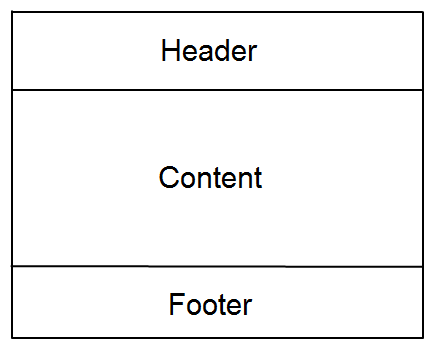
\includegraphics[width=0.3\textwidth]{Grafiken/Template.png}
			\caption{Standard-Template für alle Facelets}
		\end{figure}
		
		\paragraph{navigation.xhtml} \hypertarget{navigation}
		RS\\
		\begin{itemize}
			\item \textbf{Beschreibung:} Hier kann, abhängig von der Benutzerrolle, durch die Seite navigiert werden.
			\item \textbf{Links:}
			\begin{itemize}
				\item Suche: Navigiert zur Kurse durchsuchen Seite. \hyperlink{search}{search.xhtml}
				\item Sprache Deutsch: Ändert die angezeigte Sprache zu Deutsch.
				\item Sprache Englisch: Ändert die angezeigte Sprache zu Englisch.
				\item Profil (Benutzer): Navigiert zum eigenen Profil. \hyperlink{profile}{profile.xhtml}
				\item Meine Kurse (Benutzer): Navigiert zur Anzeige der eigenen Kurse. \hyperlink{myCourses}{myCourses.xhtml}
				\item Terminplaner (Benutzer): Navigiert zum persönlichen Terminplaner. \hyperlink{scheduler}{scheduler.xhtml}
				\item Seitenverwaltung (Administrator): Lässt den Seitenadministrator zur Seitenverwaltung navigieren. \hyperlink{adminManagement}{adminManagement.xhtml}
				\item Benutzer aktivieren: (Kursleiter, Administrator): Navigiert zur Benutzer aktivieren Seite. \hyperlink{activateUsers}{activateUsers.xhtml}
			\end{itemize}
			\begin{center}
				\begin{longtable}{|p{4cm} |p{6cm} |}

					\hline \multicolumn{1}{|c|}{\textbf{Link}} & \multicolumn{1}{|c|}{\textbf{\"{U}bergabeparameter}} \\ \hline
					\endfirsthead
					\hline
					\endlastfoot

					\textit{Suche} & -\\ \hline
					\textit{Sprache Deutsch} & language\\ \hline
					\textit{Sprache Englisch} & language\\ \hline
					\textit{Profil (B)} & -\\ \hline
					\textit{Meine Kurse (B)} & -\\ \hline
					\textit{Terminplaner (B)} & -\\ \hline
					\textit{Seitenverwaltung (A)} & -\\ \hline
					\textit{Benutzer aktivieren (K, A)} & -\\ \hline
				\end{longtable}
			\end{center}

			\item \textbf{Buttons:}
				\begin{itemize}
					\item Logout (Benutzer, wenn eingeloggt): Loggt den aktuellen eingeloggten Benutzer aus. \\ Zugehörige Methode: logout()
					\item Anmelden (Anonym): Navigiert zur Registrierungs- und Anmeldeseite. \hyperlink{authenticate}{authenticate.xhtml} \\ Zugehörige Methode: login()
				\end{itemize}
				\begin{center}
					\begin{longtable}{|p{4cm} |p{4cm} | p{4cm}|}
					
						\hline \multicolumn{1}{|c|}{\textbf{Button}} & \multicolumn{1}{|c|}{\textbf{Methode}} \\ \hline
						\endfirsthead
						\hline
						\endlastfoot
					
							\textit{Logout (B)} & logout()\\ \hline
							\textit{Anmelden} & login()\\ \hline
					\end{longtable}
				\end{center}
			\item \textbf{Inputs:} -
			\item \textbf{Outputs:}
				\begin{itemize}
					\item Logo: Zeigt verkleinertes, vom Administrator definiertes Logo der Website. Beim klick gelangt der Nutzer zur Startseite \hyperlink{index}{index.xhtml}.
				\end{itemize}
				\begin{center}
					\begin{longtable}{|p{5cm} | p{4cm}|p{3cm}|}
						
						\hline \multicolumn{1}{|c|}{\textbf{Ausgabefeld}} & \multicolumn{1}{|c|}{\textbf{Typ}}  &  \multicolumn{1}{|c|}{\textbf{ID}} \\ \hline
						\endfirsthead
						\hline
						\endlastfoot
						\textit{Logo}  & graphicImage & logo \\ \hline
					\end{longtable}
				\end{center}
			\item \textbf{BackingBean:}
				\begin{itemize}
					\item NavigationBean
				\end{itemize}
		\end{itemize}
		
		\paragraph{footer.xhtml} \hypertarget{footer}
		RS\\
		\begin{itemize}
			\item \textbf{Beschreibung:} Dieses Facelet dient der Darstellung des Footers.
			\item \textbf{Links:} -
			\item \textbf{Buttons:}
			\begin{itemize}
				\item AGB: Navigiert zum Facelet mit den Allgemeinen Geschäftsbedingungen, also \hyperlink{agb}{agb.xhtml}. Zugehörige Methode: loadAGBPage()
				\item Impressum: Navigiert zum Facelet mit dem Impressum der Webanwendung, also \hyperlink{imprint}{imprint.xhtml}. Zugehörige Methode: loadImprintPage()
				\item Hilfe: Navigiert zur Hilfeseite, also COMPLETEuserHelp.html. Zugehörige Methode: loadHelpPage()
			\end{itemize}
			\begin{center}
				\begin{longtable}{|p{4cm} |p{4cm} | p{4cm}|}
					
					\hline \multicolumn{1}{|c|}{\textbf{Button}} & \multicolumn{1}{|c|}{\textbf{Methode}}\\ \hline
					\endfirsthead
					\hline
					\endlastfoot
						\textit{AGB} & loadAGBPage()\\ \hline
						\textit{Impressum} & loadImprintPage()\\ \hline
						\textit{Hilfe} & loadHelpPage()\\ \hline
				\end{longtable}
			\end{center}
			\item \textbf{Inputs:} -
			\item \textbf{Outputs:} -
			\item \textbf{BackingBean:}
			\begin{itemize}
				\item FooterBean
			\end{itemize}
		\end{itemize}
		
		\paragraph{template.xhtml} \hypertarget{template}
		RS\\
		\begin{itemize}
			\item \textbf{Beschreibung:} Dieses Facelet dient der einheitlichen Darstellung und Struktur aller Facelets im System. Letztere ist in Abbildung 5.1 genauer dargestellt.
			\item \textbf{Links:} -
			\item \textbf{Buttons:} -
			\item \textbf{Inputs:}
			\begin{itemize}
				\item Navigation: Bindet \hyperlink{navigation}{navigation.xhtml} in den Header ein.
				\item Footer: Bindet \hyperlink{footer}{footer.xhtml} in den Footer ein.
			\end{itemize}
			\begin{center}
				\begin{longtable}{|p{3cm} |p{5cm} | p{4cm}|}
						
					\hline \multicolumn{1}{|c|}{\textbf{Eingabefeld}} & \multicolumn{1}{|c|}{\textbf{Typ}}  &  \multicolumn{1}{|c|}{\textbf{ID}} \\ \hline
					\endfirsthead
					\hline
					\endlastfoot
					\textit{Navigation} & xhtml & header \\ \hline
					\textit{Footer} & xhtml & footer \\ \hline
				\end{longtable}
			\end{center}
			\item \textbf{Outputs:} -
			\item \textbf{BackingBean:} -
		\end{itemize}
		
		\section{Facelets}
		
		\subsection{open}
		
		\subsubsection{common}
		
		\paragraph{errorPage.xhtml} \hypertarget{errorPage}
		KH\\
			\begin{itemize}
				\item \textbf{Beschreibung:} Der Benutzer wird auf diese Seite weitergeleitet, wenn Exceptions auftreten, auf die der Nutzer keinen Einfluss hat. Die entsprechende Fehlermeldung wird dann angezeigt.
				\item \textbf{Links:}
					\begin{itemize}
						\item Startseite: Über diesen Link gelangt der Benutzer zurück zur Startseite. (\hyperlink{index}{index.xhtml})
					\end{itemize}
					
					\begin{center}
						\begin{longtable}{|p{4cm} |p{6cm} |}
							
							\hline \multicolumn{1}{|c|}{\textbf{Link}} & \multicolumn{1}{|c|}{\textbf{\"{U}bergabeparameter}} \\ \hline
							\endfirsthead
							\hline
							\endlastfoot
							
							\textit{Startseite } & - \\ \hline
						\end{longtable}
					\end{center}
						
			\end{itemize}
		
		\paragraph{index.xhtml} \hypertarget{index}
		RS\\
		\begin{itemize}
			\item \textbf{Beschreibung:} Dieses Facelet stellt die Startseite des Systems dar.
			\item \textbf{Links:}
			\begin{itemize}
				\item Gesamtes Kursangebot, \hyperlink{search}{search.xhtml}
			\end{itemize}
			\item \textbf{Buttons:} -
			\item \textbf{Inputs:} -
			\item \textbf{Outputs:}
			\begin{itemize}
				\item Logo der Website
			\end{itemize}
					\begin{center}
						\begin{longtable}{|p{5cm} | p{4cm}|p{3cm}|}
							
							\hline \multicolumn{1}{|c|}{\textbf{Ausgabefeld}} & \multicolumn{1}{|c|}{\textbf{Typ}}  &  \multicolumn{1}{|c|}{\textbf{ID}} \\ \hline
							\endfirsthead
							\hline
							\endlastfoot
							\textit{Logo der Website}  & graphicImage & biglogo \\ \hline
						\end{longtable}
					\end{center}
			\item \textbf{BackingBean:} -
		\end{itemize}
		
		\paragraph{authenticate.xhtml} \hypertarget{authenticate}
		KH\\
		\begin{itemize}
			\item \textbf{Beschreibung:}
			Auf dieser Seite kann man sich im System anmelden, ein neues Benutzerkonto generieren oder ein neues Passwort anfordern.
			\item \textbf{Buttons:}
			\begin{itemize}
				\item Registrieren: Durch Drücken dieses Buttons wird der neue Benutzer mit den eingegebenen Daten im System gespeichert und es wird eine Bestätigungsmail mit dem Verifizierungslink an die angegebene E-Mail-Adresse verschickt, sofern alle Daten korrekt eingegeben wurden. \\ Zugehörige Methode: registerUser()
				\item Anmelden: Durch Drücken dieses Buttons wird der registrierte Benutzer im System angemeldet und auf die Seite 'Meine Kurse' (\hyperlink{myCourses}{myCourses.xhtml}) weitergeleitet, sofern Benutzername und Passwort korrekt eingegeben wurden. \\ Zugehörige Methode: login()
				\item Passwort vergessen: Durch Drücken dieses Buttons wird an die angegebene E-Mail-Adresse ein automatisch generiertes Passwort geschickt, sofern die Adresse im System existiert. \\ Zugehörige Methode: resetPassword()
			\end{itemize}
			
			\begin{center}
				\begin{longtable}{|p{4cm} |p{4cm} | p{4cm}|}
					
					\hline \multicolumn{1}{|c|}{\textbf{Button}} & \multicolumn{1}{|c|}{\textbf{Methode}} & \multicolumn{1}{|c|}{\textbf{\"{U}bergabeparameter}} \\ \hline
					\endfirsthead
					\hline
					\endlastfoot
					
						\textit{Registrieren } & registerUser() & - \\ \hline
						\textit{Anmelden } & login() & - \\ \hline
						\textit{Passwort vergessen } & resetPassword() & - \\ \hline
				\end{longtable}
			\end{center}
			
			\item \textbf{Inputs:}
			\begin{itemize}
				\item Anrede (Registrierung): Hier wählt der Benutzer die Anrede 'Herr' oder 'Frau' aus.
				\item Vorname (Registrierung): Hier trägt der Benutzer seinen Vornamen ein.
				\item Name (Registrierung): Hier gibt der Benutzer seinen Namen ein.
				\item Benutzername (Registrierung): Hier gibt der Benutzer einen Benutzernamen ein.
				\item Passwort (Registrierung): Hier trägt der Benutzer ein Passwort ein.
				\item Passwort bestätigen (Registrierung): Hier gibt der Benutzer das gleiche Passwort erneut ein zur Bestätigung.
				\item Geburtstag (Registrierung): Hier gibt der Benutzer sein Geburtsdatum ein.
				\item Straße (Registrierung): Hier gibt der Benutzer seine Straße ein.
				\item Hausnummer (Registrierung): Hier gibt der Benutzer seine Hausnummer ein.
				\item Stadt (Registrierung): Hier trägt der Benutzer seine Stadt ein.
				\item Postleitzahl (Registrierung): Hier trägt der Benutzer seine Postleitzahl ein.
				\item Land (Registrierung): Hier trägt der Benutzer sein Heimatland ein.
				\item E-Mail-Adresse (Registrierung): Hier gibt der Benutzer seine E-Mail-Adresse ein.
				\item AGBs bestätigen (Registrierung): Durch Setzten des Häkchens bestätigt der Benutzer die AGBs. 
				\item Benutzername (Anmeldung): Der Benutzer gibt seinen Benutzernamen ein, mit dem er sich registriert hat.
				\item Passwort (Anmeldung): Der Benutzer gibt sein Passwort ein, mit dem er sich registriert hat.
				\item E-Mail-Adresse (Passwort vergessen): Der Benutzer gibt seine im System bereits gespeicherte E-Mailadresse ein.
				
				\begin{center}
					\begin{longtable}{|p{3cm} |p{5cm} | p{4cm}|p{3cm}|}
						
						\hline \multicolumn{1}{|c|}{\textbf{Eingabefeld}} & \multicolumn{1}{|c|}{\textbf{Backing-Bean-Attribute}} & \multicolumn{1}{|c|}{\textbf{Typ}}  &  \multicolumn{1}{|c|}{\textbf{ID}} \\ \hline
						\endfirsthead
						\hline
						\endlastfoot
							\textit{Anrede (Registrierg)} & - & selectOneMenu & anrede \\ \hline
							\textit{Vorname (Registrierg)} & - & inputText & vorname \\ \hline
							\textit{Name (Registrierg)} & - & inputText & name \\ \hline
							\textit{Benutzername (Registrierg)} & - & inputText & benutzername\\ \hline
							\textit{Passwort (Registrierg)} & - & inputSecret & passwort \\ \hline
							\textit{Passwort bestätigen (Registrierg)} &- & inputSecret & bestätigungs- passwort\\ \hline
							\textit{Geburtstag (Registrierg)} & - & inputText & geburtstag \\ \hline
							\textit{Straße (Registrierg)} & - & inputText & straße\\ \hline
							\textit{Hausnummer (Registrierg)} & - & inputText & hausnummer\\ \hline
							\textit{Stadt (Registrierg)} & - & inputText & stadt \\ \hline
							\textit{Postleitzahl (Registrierg)} & - & inputText & postleitzahl \\ \hline
							\textit{Land (Registrierg)} & - & inputText & land \\ \hline
							\textit{E-Mail-Adresse (Registrierg)} & - & inputText & mail\\ \hline
							\textit{AGBs bestätigen (Registrierg)} & - & selectBooleanCheckbox & agb \\ \hline
							\textit{Benutzername (Anmeldung)} & - & inputText & anmeldungs- benutzername \\ \hline
							\textit{Passwort (Anmeldung)} & - & inputSecret & anmeldungs- passwort \\ \hline
							\textit{E-Mail-Adresse (Passwort vergessen)} & - & inputText & Passwortmail \\ \hline
					\end{longtable}
				\end{center}
				
				\begin{center}
					\begin{longtable}{|p{3cm} |p{8cm} | p{5cm}|}
						
						\hline \multicolumn{1}{|c|}{\textbf{Eingabefeld}} & \multicolumn{1}{|c|}{\textbf{Validator}} & \multicolumn{1}{|c|}{\textbf{Konverter}} \\ \hline
						\endfirsthead
						\hline
						\endlastfoot
						\textit{Anrede (Registrierg)} & - & -  \\ \hline
						\textit{Vorname (Registrierg)} & validateLength (min = 0, max = 100) & - \\ \hline
						\textit{Name (Registrierg)} & validateLength (min = 0, max =100) & -  \\ \hline
						\textit{Benutzername (Registrierg)} & UserNameValidator, validateLength (min = 5 , max =100), validateRequired  & - \\ \hline
						\textit{Passwort (Registrierg)} & PasswordValidator (mindestens 8 Zeichen, mind. 1 Sonderzeichen, mind. 1 Ziffer, Groß- und Kleinbuchstaben, keine Umlaute, kein 'ß'), validateRequired & -  \\ \hline
						\textit{Passwort bestätigen (Registrierg)} & confirmPasswordValidator, validateRequired & - \\ \hline
						\textit{Geburtstag (Registrierg)} & DateOfBirthValidator & convertDateTime  \\ \hline
						\textit{Straße (Registrierg)} & validateLength (min = 0, max = 100) & - \\ \hline
						\textit{Hausnummer (Registrierg)} & validateLength (min = 0, max = 9) & - \\ \hline
						\textit{Stadt (Registrierg)} & validateLength (min = 1, max = 100), validateRequired & -  \\ \hline
						\textit{Postleitzahl (Registrierg)} & validateLength (min = 1, max = 10), validateRequired & - \\ \hline
						\textit{Land (Registrierg)} & validateLength (min = 1, max = 100), validateRequired & -  \\ \hline
						\textit{E-Mail-Adresse (Registrierg)} & EMailValidator, validateLength (min = 1, max = 319), validateRequired & - \\ \hline
						\textit{AGBs bestätigen (Registrierg)} & - & -  \\ \hline
						\textit{Benutzername (Anmeldung)} & validateRequired & - \\ \hline
						\textit{Passwort (Anmeldung)} & validateRequired & -  \\ \hline
						\textit{E-Mail-Adresse (Passwort vergessen)} & validateRequired & - \\ \hline
					\end{longtable}
				\end{center}
				
				
			\end{itemize}
			\item \textbf{Outputs:} 
			\begin{itemize}
				\item Anrede Fehlermeldung (Registrierung): Ausgabe der Fehlermeldungen zu den Validatoren des Eingabefeldes.
				\item Vorname Fehlermeldung (Registrierung): Ausgabe der Fehlermeldungen zu den Validatoren des Eingabefeldes.
				\item Name Fehlermeldung (Registrierung): Ausgabe der Fehlermeldungen zu den Validatoren des Eingabefeldes.
				\item Benutzername Fehlermeldung (Registrierung): Ausgabe der Fehlermeldungen zu den Validatoren des Eingabefeldes.
				\item Passwort Fehlermeldung (Registrierung): Ausgabe der Fehlermeldungen zu den Validatoren des Eingabefeldes.
				\item Passwort bestätigen Fehlermeldung (Registrierung): Ausgabe der Fehlermeldungen zu den Validatoren des Eingabefeldes.
				\item Geburtstag Fehlermeldung (Registrierung): Ausgabe der Fehlermeldungen zu den Validatoren des Eingabefeldes.
				\item Straße Fehlermeldung (Registrierung): Ausgabe der Fehlermeldungen zu den Validatoren des Eingabefeldes.
				\item Hausnummer Fehlermeldung (Registrierung): Ausgabe der Fehlermeldungen zu den Validatoren des Eingabefeldes.
				\item Stadt Fehlermeldung (Registrierung): Ausgabe der Fehlermeldungen zu den Validatoren des Eingabefeldes.
				\item Postleitzahl Fehlermeldung (Registrierung): Ausgabe der Fehlermeldungen zu den Validatoren des Eingabefeldes.
				\item Land Fehlermeldung (Registrierung): Ausgabe der Fehlermeldungen zu den Validatoren des Eingabefeldes.
				\item E-Mail-Adresse Fehlermeldung (Registrierung): Ausgabe der Fehlermeldungen zu den Validatoren des Eingabefeldes.
				\item AGBs bestätigen Fehlermeldung (Registrierung): Ausgabe der Fehlermeldungen zu den Validatoren des Eingabefeldes.
				\item Benutzername Fehlermeldung (Anmeldung): Ausgabe der Fehlermeldungen zu den Validatoren des Eingabefeldes.
				\item Passwort Fehlermeldung (Anmeldung): Ausgabe der Fehlermeldungen zu den Validatoren des Eingabefeldes.
				\item E-Mail-Adresse Fehlermeldung (Passwort vergessen): Ausgabe der Fehlermeldungen zu den Validatoren des Eingabefeldes.
			\end{itemize}
			
				\begin{center}
					\begin{longtable}{|p{5cm} | p{4cm}|p{5cm}|}
						
						\hline \multicolumn{1}{|c|}{\textbf{Ausgabefeld}} & \multicolumn{1}{|c|}{\textbf{Typ}}  &  \multicolumn{1}{|c|}{\textbf{ID}} \\ \hline
						\endfirsthead
						\hline
						\endlastfoot
						\textit{Anrede Fehlermeldung (R)}  & outputText & anredefehler \\ \hline
						\textit{Vorname Fehlermeldung (R)}  & outputText & vornamenfehler \\ \hline
						\textit{Name Fehlermeldung (R)} & outputText & namenfehler \\ \hline
						\textit{Benutzername Fehlermeldung (R)}& outputText & nutzernamenfehler\\ \hline
						\textit{Passwort Fehlermeldung (R)}& outputText & passwortfehler\\ \hline
						\textit{Passwort bestätigen Fehlermeldung (R)}& outputText & bestätigungspwfehler\\ \hline
						\textit{Geburtstag  Fehlermeldung(R)} & outputText & geburtstagsfehler \\ \hline
						\textit{Straße Fehlermeldung (R)}& outputText & straßenfehler\\ \hline
						\textit{Hausnummer Fehlermeldung (R)}& outputText & hausnrfehler\\ \hline
						\textit{Stadt Fehlermeldung (R)}& outputText & stadtfehler \\ \hline
						\textit{Postleitzahl Fehlermeldung (R)} & outputText & postleitzahlfehler \\ \hline
						\textit{Land Fehlermeldung (R)} & outputText & landfehler \\ \hline
						\textit{E-Mail-Adresse Fehlermeldung (R)} & outputText & mailfehler\\ \hline
						\textit{AGBs bestätigen Fehlermeldung (R)} & outputText & agbfehler \\ \hline
						\textit{Benutzername Fehlermeldung (A)}& outputText & anmeldenamefehler \\ \hline
						\textit{Passwort Fehlermeldung (A)} &  outputText & anmeldepwfehler \\ \hline
						\textit{E-Mail-Adresse Fehlermeldung (Passwort vergessen)}  & outputText & mailpw \\ \hline
					\end{longtable}
				\end{center}
			
			\item \textbf{BackingBean:}
				\begin{itemize}
					\item AuthenticateUserBean
					\item RegisterUserBean
					\item LostPasswordBean
				\end{itemize}
		\end{itemize}
		
		\paragraph{imprint.xhtml} \hypertarget{imprint}
		KH\\
		\begin{itemize}
			\item \textbf{Beschreibung:} Auf dieser Seite kann das Impressum angezeigt werden.
			\item \textbf{Outputs:} 
				\begin{itemize}
					\item	Anzeige des Impressums, welches vom Administrator festgelegt wurde.
				\end{itemize}
				
				\begin{center}
					\begin{longtable}{|p{5cm} | p{4cm}|p{3cm}|}
						
						\hline \multicolumn{1}{|c|}{\textbf{Ausgabefeld}} & \multicolumn{1}{|c|}{\textbf{Typ}}  &  \multicolumn{1}{|c|}{\textbf{ID}} \\ \hline
						\endfirsthead
						\hline
						\endlastfoot
						\textit{Impressum}  & outputText & impressumzeigen \\ \hline
					\end{longtable}
				\end{center}
		\end{itemize}
		
		\paragraph{agb.xhtml} \hypertarget{agb}
		RS\\
		\begin{itemize}
			\item \textbf{Beschreibung:} Dieses Facelet dient der Anzeige der Allgemeinen Geschäftsbedingungen.
			\item \textbf{Links:} -
			\item \textbf{Buttons:} -
			\item \textbf{Inputs:} -
			\item \textbf{Outputs:}
			\begin{itemize}
				\item von Betreibern festgelegte Allgemeine Geschäftsbedingungen.
			\end{itemize}
				\begin{center}
					\begin{longtable}{|p{5cm} | p{4cm}|p{3cm}|}
						
						\hline \multicolumn{1}{|c|}{\textbf{Ausgabefeld}} & \multicolumn{1}{|c|}{\textbf{Typ}}  &  \multicolumn{1}{|c|}{\textbf{ID}} \\ \hline
						\endfirsthead
						\hline
						\endlastfoot
						\textit{AGB}  & outputText & agbzeigen \\ \hline
					\end{longtable}
				\end{center}
			\item \textbf{BackingBean:} -
		\end{itemize}
		
		
		\subsubsection{courses}
		
		\paragraph{search.xhtml} \hypertarget{search}
		RS\\
		\begin{itemize}
			\item \textbf{Beschreibung:} Hier können alle Kurse angezeigt und durchsucht werden.
			\item \textbf{Links:} -
			\item \textbf{Buttons:}
			\begin{itemize}
				\item Anzeigen: Zeigt die Angebote im ausgewählten Zeitraum an. \\ Zugehörige Methode: displayCoursesInSpecificPeriod()
				\item Suchen: Durchsucht die Website nach dem eingegebenen Suchbegriff mittels gewählten Suchobjekt. \\ Zugehörige Methode: search()
				\item Details: Navigiert den Nutzer zur jeweiligen Kursdetailseite. (\hyperlink{courseDetails}{courseDetails.xhtml}) \\
				Zugehörige Methode: loadCourseDetailsPageOfSelectedCourse()
			\end{itemize}
			\begin{center}
				\begin{longtable}{|p{2cm} |p{9cm} | p{4cm}|}
						
					\hline \multicolumn{1}{|c|}{\textbf{Button}} & \multicolumn{1}{|c|}{\textbf{Methode}} & \multicolumn{1}{|c|}{\textbf{\"{U}bergabeparameter}}\\ \hline
					\endfirsthead
					\hline
					\endlastfoot
			
					\textit{Anzeigen} & displayCoursesInSpecificPeriod() & timespan\\ \hline
					\textit{Suchen} &  search() & searched\\ \hline
					\textit{Details} & loadCourseDetailsPageOfSelectedCourse() & courseid\\ \hline
				\end{longtable}
			\end{center}
			\item \textbf{Inputs:}
			\begin{itemize}
				\item Angebotszeitraum: Ermöglicht eine genauere Anzeige des Kursangebots, entweder Tagesangebot, Wochenangebot oder das gesamte Angebot. Die detaillierteren Suchoptionen sind nur für registrierte Benutzer verfügbar.
				\item Suchobjekt (abhängig von Benutzerrolle): Ermöglicht eine genauere Suche, beispielsweise nach Kursen, Kursleitern oder Kurs-ID.
			\end{itemize}
				\begin{center}
					\begin{longtable}{|p{3cm} |p{4cm} | p{4cm}|p{3cm} |p{2cm}|}
						
						\hline \multicolumn{1}{|c|}{\textbf{Feld}} & \multicolumn{1}{|c|}{\textbf{Action}} & \multicolumn{1}{|c|}{\textbf{Validatoren}}  &  \multicolumn{1}{|c|}{\textbf{ID}} \\ \hline
						\endfirsthead
						\hline
						\endlastfoot
						\textit{Angebots-zeitraum} & setDisplayPeriod() & validateRequired & time\\ \hline
						\textit{Suchobjekt} & setSearchParam() & validateRequired & searchparam\\ \hline
					\end{longtable}
				\end{center}
			\item \textbf{Outputs:}
			\begin{itemize}
				\item Tabelle mit Ergebnissen der Suche.
				\item Schaltfläche um zwischen Ergebnissen zu Blättern.
			\end{itemize}
					\begin{center}
						\begin{longtable}{|p{5cm} | p{4cm}|p{3cm}|}
							
							\hline \multicolumn{1}{|c|}{\textbf{Ausgabefeld}} & \multicolumn{1}{|c|}{\textbf{Typ}}  &  \multicolumn{1}{|c|}{\textbf{ID}} \\ \hline
							\endfirsthead
							\hline
							\endlastfoot
							\textit{Suchtabelle}  & dataTable & searchtable \\ \hline
							\textit{Schaltfläche}  & panelGroup & pagenav \\ \hline
						\end{longtable}
					\end{center}
			\item \textbf{BackingBean:}
			\begin{itemize}
				\item SearchCourseBean
			\end{itemize}
		\end{itemize}
		
		\paragraph{courseDetails.xhtml} \hypertarget{courseDetails}
		RS\\
		\begin{itemize}
			\item \textbf{Beschreibung:} Zur genaueren Betrachtung eines einzelnen Kurses wird dieses Facelet benötigt.
			\item \textbf{Links:} -
			\item \textbf{Buttons:}
			\begin{itemize}
				\item Anmelden (Benutzer, noch nicht angemeldet): Meldet den Benutzer zum Kurs an. \\ Zugehörige Methode: signUpForCourse()
				\item Abmelden (Benutzer, wenn angemeldet): Meldet den Benutzer vom Kurs ab. \\ Zugehörige Methode: signOffFromCourse()
				\item Teilnehmer anzeigen (Benutzer): Zeigt die zum Kurs angemeldeten Benutzer an. \hyperlink{listParticipants}{listParticipants.xhtml} \\ Zugehörige Methode: loadParticipantsPage()
				\item Alle auswählen (Benutzer, zum Kurs angemeldet): Wählt alle Kurseinheiten des Kurses aus. \\ Zugehörige Methode: selectAllCourseUnits()
				\item Speichern (Benutzer, zum Kurs angemeldet): Speichert alle ausgewählten Kurseinheiten und meldet den Nutzer dazu an. \\ Zugehörige Methode: signUpForCourseUnits()
				\item Bearbeiten (Administrator, noch nicht im Bearbeitungsmodus): Ermöglicht die Bearbeitung der einzelnen Kursdetails. \\ Zugehörige Methode: editCourse()
				\item Speichern (Administrator, im Bearbeitungsmodus): Speichert alle vorgenommenen Kursänderungen. \\ Zugehörige Methode: saveCourse()
				\item Hinzufügen (Administrator): Fügt einen Kursleiter zum Kurs hinzu. Zugehörige Methode: addCourseLeader()
				\item Kurseinheit anlegen (Kursleiter): Erstellt eine neue Kurseinheit zum Kurs. \hyperlink{editCourseUnit}{editCourseUnit.xhtml} \\ Zugehörige Methode: loadCreateCourseUnitPage()
				\item Kurseinheit bearbeiten (Kursleiter): Ermöglicht die Bearbeitung einer einzelnen Kurseinheit. \hyperlink{editCourseUnit}{editCourseUnit.xhtml} \\ Zugehörige Methode: loadEditCourseUnitPage()
				\item Kurs löschen (Administrator): Löscht den Kurs. \\ Zugehörige Methode: deleteCourse()
			\end{itemize}
			\begin{center}
				\begin{longtable}{|p{4cm} |p{6cm} | p{4cm}|}
						
					\hline \multicolumn{1}{|c|}{\textbf{Button}} & \multicolumn{1}{|c|}{\textbf{Methode}} & \multicolumn{1}{|c|}{\textbf{\"{U}bergabeparameter}} \\ \hline
					\endfirsthead
					\hline
					\endlastfoot
			
					\textit{Anmelden (B)} & signUpForCourse() & - \\ \hline
					\textit{Abmelden (B)} &  signOffFromCourse() & - \\ \hline
					\textit{Teilnehmer anzeigen (B)} & loadParticipantsPage() & courseid \\ \hline
					\textit{Alle auswählen (B)} & selectAllCourseUnits() & - \\ \hline
					\textit{Speichern (B)} & signUpForCourseUnits() & courseids \\ \hline
					\textit{Bearbeiten (A)} & editCourse() & - \\ \hline
					\textit{Speichern (A)} & saveCourse() & - \\ \hline
					\textit{Hinzufügen (A)} & addCourseLeader() & - \\ \hline
					\textit{Kurseinheit anlegen (K)} & loadCreateCourseUnitPage() & courseid \\ \hline
					\textit{Kurseinheit bearbeiten (K)} & loadEditCourseUnitPage() & courseunitid \\ \hline
					\textit{Kurs löschen (A)} & deleteCourse() & - \\ \hline
				\end{longtable}
			\end{center}
			\item \textbf{Inputs:}
			\begin{itemize}
				\item Kursnews erhalten: Trägt Benutzer bei Anmeldung zum Kurs in die Kursnews ein.
				\item Kurseinheit auswählen: Wählt Kurseinheit aus, zu der sich der Nutzer anmelden möchte.
				\item Kursleiter auswählen (Administrator): Wählt Kursleiter aus, welcher gelöscht werden soll.
				\item Kursleiter Name (Administrator): Eingabefeld für den Namen eines neuen Kursleiters.
				\item Kursleiter E-Mail (Administrator): Eingabefeld für die E-Mail Adresse eines neuen Kursleiters.
				\item Kursbeschreibung (Administrator): Eingabefeld für die Kursbeschreibung.
				\item Maximale Teilnehmerzahl (Administrator): Eingabefeld für die maximale Teilnehmerzahl des Kurses.
				\item Startdatum (Administrator): Eingabefeld für das Startdatum des Kurses.
				\item Enddatum (Administrator): Eingabefeld für das Enddatum des Kurses.
			\end{itemize}
				\begin{center}
					\begin{longtable}{|p{3cm} |p{9cm} |}
						
						\hline \multicolumn{1}{|c|}{\textbf{Feld}} & \multicolumn{1}{|c|}{\textbf{Backing-Bean-Attribute}}\\ \hline
						\endfirsthead
						\hline
						\endlastfoot
						\textit{Kursnews erhalten} & CourseDetailBean.registeredForCourseNews\\ \hline
						\textit{Kurseinheit auswählen} & CourseDetailBean.selectedCourseUnits\\ \hline
						\textit{Kursleiter auswählen (A)} & CourseDetailBean.leadersOfCourse\\ \hline
						\textit{Kursleiter Name (A)} & CourseDetailBean.leadersOfCourse.User.lastname\\ \hline
						\textit{Kursleiter E-Mail (A)} & CourseDetailBean.leadersOfCourse.User.email\\ \hline
						\textit{Kursbeschreibung (A)} & CourseDetailBean.Course.description\\ \hline
						\textit{Maximale Teilnehmerzahl (A)} & CourseDetailBean.Course.maxUsers\\ \hline
						\textit{Startdatum (A)} & CourseDetailBean.Course.startdate\\ \hline
						\textit{Enddatum (A)} & CourseDetailBean.Course.enddate\\ \hline
					\end{longtable}
					\begin{longtable}{|p{3cm} |p{4cm} | p{4cm}|p{3cm} ||}
						
						\hline \multicolumn{1}{|c|}{\textbf{Feld}} & \multicolumn{1}{|c|}{\textbf{Validatoren}}  &  \multicolumn{1}{|c|}{\textbf{Konverter}} &  \multicolumn{1}{|c|}{\textbf{ID}} \\ \hline
						\endfirsthead
						\hline
						\endlastfoot
						\textit{Kursnews erhalten} & - & - & getcnews\\ \hline
						\textit{Kurseinheit auswählen} & - & - & selectcunit\\ \hline
						\textit{Kursleiter auswählen (A)} & - & - & selectcleader\\ \hline
						\textit{Kursleiter Name (A)} & - & - & cleadername\\ \hline
						\textit{Kursleiter E-Mail (A)} & - & - & cleadermail\\ \hline
						\textit{Kursbeschreibung (A)} & - & - & cdetails\\ \hline
						\textit{Maximale Teilnehmerzahl (A)} & - & convertNumber & maxparticipants\\ \hline
						\textit{Startdatum (A)} & DateValidator & convertDateTime & begin\\ \hline
						\textit{Enddatum (A)} & DateValidator & convertDateTime & end\\ \hline
					\end{longtable}
				\end{center}
			\item \textbf{Outputs:}
			\begin{itemize}
				\item Tabelle Kursleiter: Tabelle mit den Kontaktinformationen der/des Kursleiters.
				\item Tabelle Kurseinheiten: Tabelle mit allen Kurseinheiten des Kurses und zugehörigen Informationen wie Ort, Preis oder Datum.
				\item Kurs-ID: Zeigt die zum Kurs zugehörige ID an.
				\item Kursbeschreibung: Zeigt die Beschreibung zum Kurs an.
				\item Maximale Teilnehmerzahl: Zeigt die für den Kurs maximale Teilnehmerzahl an.
				\item Fehlermeldung zu den einzelnen Eingabefeldern, bei falscher Eingabe.
			\end{itemize}
					\begin{center}
						\begin{longtable}{|p{5cm} | p{4cm}|p{3cm}|}
							
							\hline \multicolumn{1}{|c|}{\textbf{Ausgabefeld}} & \multicolumn{1}{|c|}{\textbf{Typ}}  &  \multicolumn{1}{|c|}{\textbf{ID}} \\ \hline
							\endfirsthead
							\hline
							\endlastfoot
							\textit{Tabelle Kursleiter}  & dataTable & kursleiter \\ \hline
							\textit{Tabelle Kurseinheiten}  & dataTable & kurseinheiten \\ \hline
							\textit{Kurs-ID}  & outputText & id \\ \hline
							\textit{Kursbeschreibung}  & outputText & beschr \\ \hline
							\textit{Minimale Teilnehmerzahl}  & outputText & minteilnehmer \\ \hline
							\textit{Maximale Teilnehmerzahl}  & outputText & maxteilnehmer \\ \hline
							\textit{Kursleiter Name Fehlermeldung}  & outputText & knamefehler \\ \hline
							\textit{Kursleiter E-Mail Fehlermeldung}  & outputText & kmailfehler \\ \hline
							\textit{Kursbeschreibung Fehlermeldung}  & outputText & beschrfehler \\ \hline
							\textit{Minimale Teilnehmerzahl Fehlermeldung}  & outputText & minteilnfehler \\ \hline
							\textit{Maximale Teilnehmerzahl Fehlermeldung}  & outputText & maxteilnfehler \\ \hline
							\textit{Startdatum Fehlermeldung}  & outputText & startdatumfehler \\ \hline
							\textit{Enddatum Fehlermeldung}  & outputText & enddatumfehler \\ \hline
						\end{longtable}
					\end{center}
			\item \textbf{BackingBean:}
			\begin{itemize}
				\item CourseDetailBean
				\item CourseManagementBean
			\end{itemize}
		\end{itemize}
		
		\subsection{users}
		
		\subsubsection{registeredUser}
		
		\paragraph{myCourses.xhtml} \hypertarget{myCourses}
		KH\\
		\begin{itemize}
			\item \textbf{Beschreibung:} Auf dieser Seite werden alle Kurse angezeigt, in die der Teilnehmer eingetragen ist.
			\item \textbf{Links:}
				\begin{itemize}
					\item Kurstitel: Über die Kurstitel gelangt der Benutzer auf die jeweilige Kursdetailseite. (\hyperlink{courseDetails}{courseDetails.xhtml})
				\end{itemize}
				
				\begin{center}
					\begin{longtable}{|p{3cm} |p{10cm} |}
						
						\hline \multicolumn{1}{|c|}{\textbf{Link}} & \multicolumn{1}{|c|}{\textbf{\"{U}bergabeparameter}} \\ \hline
						\endfirsthead
						\hline
						\endlastfoot
						
						\textit{Kurstitel } & courseId (Id des ausgewählten Kurses wird übergeben)\\ \hline
					\end{longtable}
				\end{center}
			\item \textbf{Button:}	
				\begin{itemize}
					\item Details: Über den Button Details hinter dem jeweiligen Kurs gelangt der Benutzer auf die jeweilige Kursdetailseite. (\hyperlink{courseDetails}{courseDetails.xhtml}) \\ zugehörige Methode: loadCourseDetailsPageOfSelectedCourse()
				\end{itemize}
				\begin{center}
					\begin{longtable}{|p{4cm} |p{6cm} | p{4cm}|}
						
						\hline \multicolumn{1}{|c|}{\textbf{Button}} & \multicolumn{1}{|c|}{\textbf{Methode}} & \multicolumn{1}{|c|}{\textbf{\"{U}bergabeparameter}} \\ \hline
						\endfirsthead
						\hline
						\endlastfoot
						
						\textit{Details} &  loadCourseDetailsPageOfSelected Course()  & courseID (Id des ausgewählten Kurses wird übergeben) \\ \hline
					\end{longtable}
				\end{center}
				
				
			\item \textbf{Outputs:}
				\begin{itemize}
					\item Tabelle Auflistung aller Kurse: Hier werden dem Benutzer alle seine angemeldeten Kurse angezeigt.
				\end{itemize}
				
				\begin{center}
					\begin{longtable}{|p{5cm} | p{4cm}|p{3cm}|}
						
						\hline \multicolumn{1}{|c|}{\textbf{Ausgabefeld}} & \multicolumn{1}{|c|}{\textbf{Typ}}  &  \multicolumn{1}{|c|}{\textbf{ID}} \\ \hline
						\endfirsthead
						\hline
						\endlastfoot
						\textit{Kurstabelle}  & dataTable & kurstabelle \\ \hline
					\end{longtable}
				\end{center}
				
			\item \textbf{BackingBean:}
				\begin{itemize}
					\item MyCoursesBean
				\end{itemize}
		\end{itemize}
		
		\paragraph{profile.xhtml} \hypertarget{profile}
		KH\\
		\begin{itemize}
			\item \textbf{Beschreibung:} Auf dieser Seite werden die persönlichen Daten und der Kontostand des Benutzers angezeigt. Erstere kann er hier ändern. Der Kursleiter kann hier den Benutzer aktivieren, und der Administrator den Benutzer löschen.
			\item \textbf{Buttons:}
				\begin{itemize}
					\item Bearbeiten: Nach Klicken auf diesen Button können die persönlichen Daten geändert werden. Der Button trägt nun die Aufschrift 'Speichern' und ist mit dessen dazugehöriger Methode hinterlegt. \\ Zugehörige Methode: editUserData()
					\item Speichern: Durch Drücken dieses Buttons werden die vorgenommenen Änderungen gespeichert, sofern alle Daten korrekt eingegeben wurden. Bei Änderung der E-Mail-Adresse wird außerdem eine Bestätigungsmail mit einem Verifizierungslink verschickt. Bei erfolgreicher Speicherung erscheint der Button 'Bearbeiten' anstelle des Button 'Speichern'. \\ Zugehörige Methode: saveUserData()
					\item Durchsuchen: Durch Drücken dieses Buttons kann das eigene Dateiverzeichnis nach einem Bild durchsucht werden.
					\item Hochladen: Durch Drücken dieses Buttons wird das ausgewählte Profilbild hochgeladen. \\ Zugehörige Methode: uploadProfilPic()  weitergeleitet.
					\item Benutzer löschen: Durch Drücken dieses Buttons entfernt der Administrator diesen Benutzer aus dem System, oder der Benutzer kann sich selbst auf inaktiv setzen. Setzt sich der Benutzer selbst auf inaktiv, so wird er auf die Startseite weitergeleitet. (\hyperlink{index}{index.xhtml})  \\ Zugehörige Methoden: deleteUser(), setUserInactive() 
				\end{itemize}
				
					\begin{center}
						\begin{longtable}{|p{4cm} |p{6cm} | p{4cm}|}
							
							\hline \multicolumn{1}{|c|}{\textbf{Button}} & \multicolumn{1}{|c|}{\textbf{Methode}} & \multicolumn{1}{|c|}{\textbf{\"{U}bergabeparameter}} \\ \hline
							\endfirsthead
							\hline
							\endlastfoot
							
							\textit{Bearbeiten } & editUserData() & - \\ \hline
							\textit{Speichern } & saveUserData() & - \\ \hline
							\textit{Duchsuchen } & - & - \\ \hline
							\textit{Hochladen } & uploadProfilPic() & - \\ \hline
							\textit{Benutzer löschen} &  deleteUser(), setUserInactive()  & - \\ \hline
						\end{longtable}
					\end{center}
				
			\item \textbf{Inputs:}
				\begin{itemize}
					\item Anrede: Hier kann der Benutzer seine Anrede ändern.
					\item Vorname: Hier kann der Benutzer seinen Vornamen ändern.
					\item Name: Hier kann der Benutzer seinen Namen ändern.
					\item Geburtstag: Hier kann der Benutzer sein Geburtsdatum ändern.
					\item Straße: Hier kann der Benutzer seine Straße ändern.
					\item Hausnummer: Hier kann der Benutzer seine Hausnummer ändern.
					\item Stadt: Hier kann der Benutzer seine Stadt ändern.
					\item Postleitzahl: Hier kann der Benutzer seine Postleitzahl ändern.
					\item Land: Hier kann der Benutzer seine Land ändern.
					\item E-Mail-Adresse: Hier kann der Benutzer seine E-Mail-Adresse ändern.
					\item Benutzername: Hier kann der Benutzer seinen Benutzernamen ändern.
					\item Passwort: Hier kann der Benutzer sein Passwort ändern.
					\item Passwort bestätigen: Hier muss der Benutzer sein geändertes Passwort bestätigen.
					\item Benutzerrolle: Hier kann der Administrator die Benutzerrolle eines Nutzers ändern.
					\item Profilbild Pfad: Hier kann der Benutzer sein Profilbild ändern.
				\end{itemize}
				
				\begin{center}
					\begin{longtable}{|p{3cm} |p{6cm} | p{4cm}|p{3cm}|}
						
						\hline \multicolumn{1}{|c|}{\textbf{Eingabefeld}} & \multicolumn{1}{|c|}{\textbf{Backing-Bean-Attribute}} & \multicolumn{1}{|c|}{\textbf{Typ}}  &  \multicolumn{1}{|c|}{\textbf{ID}} \\ \hline
						\endfirsthead
						\hline
						\endlastfoot
						\textit{Anrede} & UserProfilBean.User.salutation & selectOneMenu & anrede \\ \hline
						\textit{Vorname} & UserProfilBean.User.fistname & inputText & vorname \\ \hline
						\textit{Name} & UserProfilBean.User.lastname & inputText & name \\ \hline
						\textit{Geburtstag } & UserProfilBean.User.dateOfBirth & inputText & geburtstag \\ \hline
						\textit{Straße} & UserProfilBean.Address.street & inputText & straße\\ \hline
						\textit{Hausnummer} & UserProfil.Address.houseNumber  & inputText & hausnummer\\ \hline
						\textit{Stadt} & UserProfilBean.Address.city & inputText & stadt \\ \hline
						\textit{Postleitzahl} & UserProfilBean.Address.zipCode & inputText & postleitzahl \\ \hline
						\textit{Land} & UserProfilBean.Address.country & inputText & land \\ \hline
						\textit{E-Mail-Adresse} & UserProfilBean.User.email & inputText & mail\\ \hline
						\textit{Benutzername} & UserProfilBean.User.username & inputText & benutzername \\ \hline
						\textit{Passwort} & UserProfilBean.User.password  & inputSecret & passwort \\ \hline
						\textit{Passwort bestätigen} & UserProfilBean.User.password & inputSecret & bestätigungs- passwort \\ \hline
						\textit{Benutzerrolle} & UserProfilBean.User.userRole & inputText & rolle \\ \hline
						\textit{Profilbild Pfad} & UserProfilBean.User.profilImage & inputFile & bildpfad \\ \hline
					\end{longtable}
				\end{center}
				
				\begin{center}
					\begin{longtable}{|p{3cm} |p{8cm} | p{5cm}|}
						
						\hline \multicolumn{1}{|c|}{\textbf{Eingabefeld}} & \multicolumn{1}{|c|}{\textbf{Validator}} & \multicolumn{1}{|c|}{\textbf{Konverter}} \\ \hline
						\endfirsthead
						\hline
						\endlastfoot
						\textit{Anrede} & - & - \\ \hline
						\textit{Vorname} & validateLength (min =0, max = 100) & - \\ \hline
						\textit{Name} & validateLength (min = 0, max = 100) & -  \\ \hline
						\textit{Geburtstag} & DateOfBirthValidator & convertDateTime  \\ \hline
						\textit{Straße} & validateLength (min = 0, max = 100) & - \\ \hline
						\textit{Hausnummer} & validateLength (min = 0, max = 9) & - \\ \hline
						\textit{Stadt} & validateLength (min = 1, max = 100), validateRequired & -  \\ \hline
						\textit{Postleitzahl} & validateLength (min = 1, max = 10), validateRequired & - \\ \hline
						\textit{Land} & validateLength (min = 1, max = 100), validateRequired & -  \\ \hline
						\textit{E-Mail-Adresse} & EMailValidator, validateLength (min = 1, max = 390), validateRequired & - \\ \hline
						\textit{Benutzername} & UserNameValidator, validateLength (min = 5, max = 100), validateRequired  & - \\ \hline
						\textit{Passwort} & PasswordValidator (mindestens 8 Zeichen, mind. 1 Sonderzeichen, mind. 1 Ziffer, Groß- und Kleinbuchstaben, keine Umlaute, kein 'ß'), validateRequired & -  \\ \hline
						\textit{Passwort bestätigen} & ConfirmPasswordValidator, validateRequired & - \\ \hline
						\textit{Benutzerrolle} & validateRequired & - \\ \hline
						\textit{Profilbild Pfad} & UserImageValidator & - \\ \hline
					\end{longtable}
				\end{center}
				
				
			\item \textbf{Outputs:}
				\begin{itemize}
					\item Benutzer-ID: Ausgabe der automatisch generierten ID.
					\item Vorname Fehlermeldung: Ausgabe der Fehlermeldungen zu den Validatoren des Eingabefeldes.
					\item Name Fehlermeldung: Ausgabe der Fehlermeldungen zu den Validatoren des Eingabefeldes.
					\item Geburtstag Fehlermeldung: Ausgabe der Fehlermeldungen zu den Validatoren des Eingabefeldes.
					\item Straße Fehlermeldung: Ausgabe der Fehlermeldungen zu den Validatoren des Eingabefeldes.
					\item Hausnummer Fehlermeldung: Ausgabe der Fehlermeldungen zu den Validatoren des Eingabefeldes.
					\item Stadt Fehlermeldung: Ausgabe der Fehlermeldungen zu den Validatoren des Eingabefeldes.
					\item Postleitzahl Fehlermeldung: Ausgabe der Fehlermeldungen zu den Validatoren des Eingabefeldes.
					\item Land Fehlermeldung: Ausgabe der Fehlermeldungen zu den Validatoren des Eingabefeldes.
					\item E-Mail-Adresse Fehlermeldung: Ausgabe der Fehlermeldungen zu den Validatoren des Eingabefeldes.
					\item Benutzername Fehlermeldung: Ausgabe der Fehlermeldungen zu den Validatoren des Eingabefeldes.
					\item Passwort Fehlermeldung: Ausgabe der Fehlermeldungen zu den Validatoren des Eingabefeldes.
					\item Passwort bestätigen Fehlermeldung: Ausgabe der Fehlermeldungen zu den Validatoren des Eingabefeldes.
					\item Profilbild Fehlermeldung: Ausgabe der Fehlermeldungen zu den Validatoren des Eingabefeldes.
					\item Kontostand: Ausgabe des aktuellen Kontostandes.
					\item Tabelle Auflistung der Trainingskurse: Hier werden dem Kursleiter alle Kurse aufgelistet, die er leitet.
					\item Profilbild: Hier wird das Profilbild angezeigt.
				\end{itemize}
				
				\begin{center}
					\begin{longtable}{|p{5cm} | p{4cm}|p{5cm}|}
						
						\hline \multicolumn{1}{|c|}{\textbf{Ausgabefeld}} & \multicolumn{1}{|c|}{\textbf{Typ}}  &  \multicolumn{1}{|c|}{\textbf{ID}} \\ \hline
						\endfirsthead
						\hline
						\endlastfoot
						\textit{Benutzer-ID}  & outputText & nutzerid \\ \hline
						\textit{Vorname Fehlermeldung }  & outputText & vornamefehler \\ \hline
						\textit{Name Fehlermeldung } & outputText & namefehler \\ \hline
						\textit{Geburtstag  Fehlermeldung} & outputText & geburtstagsfehler \\ \hline
						\textit{Straße Fehlermeldung }& outputText & straßefehler\\ \hline
						\textit{Hausnummer Fehlermeldung }& outputText & hausnrfehler\\ \hline
						\textit{Stadt Fehlermeldung }& outputText & stadtfehler \\ \hline
						\textit{Postleitzahl Fehlermeldung } & outputText & postleitzahlfehler \\ \hline
						\textit{Land Fehlermeldung } & outputText & landfehler \\ \hline
						\textit{E-Mail-Adresse Fehlermeldung} & outputText & mailfehler\\ \hline
						\textit{Benutzername Fehlermeldung }& outputText & nutzernamefehler \\ \hline
						\textit{Passwort Fehlermeldung} &  outputText & passwortfehler \\ \hline
						\textit{Passwort bestätigen Fehlermeldung}  & outputText & bestätigungspwfehler \\ \hline
						\textit{Profilbild Fehlermeldung} &  outputText & bildfehler \\ \hline
						\textit{Kontostand} &  outputText & kontostand \\ \hline
						\textit{Tabelle Trainingskurse} &  dataTable & trainingskurse \\ \hline
						\textit{Profilbild} &  graphicImage & bild \\ \hline
					\end{longtable}
				\end{center}
				
			\item \textbf{BackingBean:}
				\begin{itemize}
					\item UserProfileBean
					\item UserManagementBean				
				\end{itemize}
		\end{itemize}
		
		\paragraph{scheduler.xhtml} \hypertarget{scheduler}
		RS\\
		\begin{itemize}
			\item \textbf{Beschreibung:} Persönlicher Terminplaner mit anstehenden Kursen.
			\item \textbf{Links:}
			\begin{itemize}
				\item Wochenansicht vorwärts: Zeigt die Termine der nächsten Woche an.
				\item Wochenansicht rückwärts: Zeigt die Termine der letzten Woche an.
			\end{itemize}
				\begin{center}
					\begin{longtable}{|p{3cm} |p{5cm} |}
						
						\hline \multicolumn{1}{|c|}{\textbf{Link}} & \multicolumn{1}{|c|}{\textbf{Methode}} \\ \hline
						\endfirsthead
						\hline
						\endlastfoot
						
						\textit{Wochenansicht vorwärts} & displayNextWeek() \\ \hline
						\textit{Wochenansicht rückwärts} & displayPreviousWeek() \\ \hline
					\end{longtable}
				\end{center}
			\item \textbf{Buttons:} -
			\item \textbf{Inputs:} -
			\item \textbf{Outputs:}
			\begin{itemize}
				\item Wochentabelle: Zeigt von Montag bis Sonntag alle belegten Kurseinheiten an. Orientiert sich am klassischen Stundenplan, also mit stündlicher Ansicht.
			\end{itemize}
				\begin{center}
					\begin{longtable}{|p{4cm} | p{3cm}|p{3cm}|}
						
						\hline \multicolumn{1}{|c|}{\textbf{Ausgabefeld}} & \multicolumn{1}{|c|}{\textbf{Typ}}  &  \multicolumn{1}{|c|}{\textbf{ID}} \\ \hline
						\endfirsthead
						\hline
						\endlastfoot
						\textit{Wochentabelle}  & dataTable & wtable \\ \hline
					\end{longtable}
				\end{center}
			\item \textbf{BackingBean:}
			\begin{itemize}
				\item SchedulerBean
			\end{itemize}
		\end{itemize}
		
		\paragraph{leaderProfile.xhtml} \hypertarget{leaderProfile}
		KH\\
		\begin{itemize}
			\item \textbf{Beschreibung:} Auf dieser Seite werden die Daten des Kursleiters, mit Ausnahme von sensiblen Daten wie Passwort oder Kontostand, und die von ihm geleiteten Kurse angezeigt.
			\item \textbf{Outputs:} 
			\begin{itemize}
				\item Tabelle Auflistung Kursleiterdaten: Hier werden die Daten des Kursleiters und die von ihm geleiteten Kurse angezeigt.
			\end{itemize}
			
			\begin{center}
				\begin{longtable}{|p{5cm} | p{4cm}|p{3cm}|}
					
					\hline \multicolumn{1}{|c|}{\textbf{Ausgabefeld}} & \multicolumn{1}{|c|}{\textbf{Typ}}  &  \multicolumn{1}{|c|}{\textbf{ID}} \\ \hline
					\endfirsthead
					\hline
					\endlastfoot
					\textit{Tabelle Kursleiterdaten}  & dataTable & kursleiterdaten \\ \hline
				\end{longtable}
			\end{center}
			
			\item \textbf{BackingBean:}
			\begin{itemize}
				\item UserProfileBean			
			\end{itemize}
		\end{itemize}
		
		\paragraph{listParticipants.xhtml} \hypertarget{listParticipants}
		KH\\
		\begin{itemize}
			\item \textbf{Beschreibung:} Hier kann der registrierte Benutzer die Teilnehmer eines Kurses mit Benutzername und Profilbild ansehen. Dem Kursleiter werden zusätzlich die E-Mail-Adresse und die Information über den Erhalt von Kursnews angezeigt. Außerdem kann er einen Teilnehmer aus dem Kurs entfernen.
			\item \textbf{Buttons:}
			\begin{itemize}
				\item Löschen: Durch Drücken dieses Buttons kann der Kursleiter den entsprechenden Benutzer aus dem Kurs entfernen. \\ Zugehörige Methode: deleteUserFromCourse()
				\item Zurück: Durch Drücken dieses Buttons kehrt der Benutzer zur entsprechenden Kursdetailseite zurück. (\hyperlink{courseDetails}{courseDetails.xhtml}) \\ Zugehörige Methode: cancel()
				
				\begin{center}
					\begin{longtable}{|p{4cm} |p{6cm} | p{4cm}|}
						
						\hline \multicolumn{1}{|c|}{\textbf{Button}} & \multicolumn{1}{|c|}{\textbf{Methode}} & \multicolumn{1}{|c|}{\textbf{\"{U}bergabeparameter}} \\ \hline
						\endfirsthead
						\hline
						\endlastfoot
						
						\textit{Löschen } & deleteUserFromCourse() & - \\ \hline
						\textit{Zurück } & cancel() & courseId (die Id des entsprechenden Kurses wird übergeben) \\ \hline
					\end{longtable}
				\end{center}
				
			\end{itemize}
			\item \textbf{Inputs:}
			\begin{itemize}
				\item Entfernen: Durch Setzen des Häkchens wählt der Kursleiter diesen Benutzer aus, um ihn anschließend über den Button 'Löschen' zu entfernen.
				
				\begin{center}
					\begin{longtable}{|p{3cm} |p{5cm} | p{4cm}|p{3cm}|}
						
						\hline \multicolumn{1}{|c|}{\textbf{Eingabefeld}} & \multicolumn{1}{|c|}{\textbf{Backing-Bean-Attribute}} & \multicolumn{1}{|c|}{\textbf{Typ}}  &  \multicolumn{1}{|c|}{\textbf{ID}} \\ \hline
						\endfirsthead
						\hline
						\endlastfoot
						\textit{Entfernen} & - & selectBooleanCheckbox & entfernen \\ \hline
					\end{longtable}
				\end{center}
				
				\begin{center}
					\begin{longtable}{|p{3cm} |p{8cm} | p{5cm}|}
						
						\hline \multicolumn{1}{|c|}{\textbf{Eingabefeld}} & \multicolumn{1}{|c|}{\textbf{Validator}} & \multicolumn{1}{|c|}{\textbf{Konverter}} \\ \hline
						\endfirsthead
						\hline
						\endlastfoot
						\textit{Entfernen} & - & - \\ \hline
					\end{longtable}
				\end{center}
				
			\end{itemize}
			\item \textbf{Outputs:} 
			\begin{itemize}
				\item Tabelle Auflistung Kursteilnehmer: Hier werden die Teilnehmer des Kurses angezeigt.
			\end{itemize}
			
			\begin{center}
				\begin{longtable}{|p{5cm} | p{4cm}|p{3cm}|}
					
					\hline \multicolumn{1}{|c|}{\textbf{Ausgabefeld}} & \multicolumn{1}{|c|}{\textbf{Typ}}  &  \multicolumn{1}{|c|}{\textbf{ID}} \\ \hline
					\endfirsthead
					\hline
					\endlastfoot
					\textit{Tabelle Kursteilnehmer}  & dataTable & kursteilnehmer \\ \hline
				\end{longtable}
			\end{center}
			
			
			\item \textbf{BackingBean:}
			\begin{itemize}
				\item ListParticipantsBean
			\end{itemize}
		\end{itemize}
		
		\subsubsection{courseLeader}
		
		\paragraph{editCourseUnit.xhtml} \hypertarget{editCourseUnit}
		KH\\
		\begin{itemize}
			\item \textbf{Beschreibung:} Auf dieser Seite können Kursleiter beziehungsweise Administratoren Kurseinheiten anlegen und bearbeiten, oder Kursteilnehmer hinzufügen und entfernen
			\item \textbf{Links:} -
			\item \textbf{Buttons:}
				\begin{itemize}
					\item Bearbeiten (Kurseinheit): Nach Klicken auf diesen Button können die Daten der Kurseinheit geändert beziehungsweise eingetragen werden. Der Button trägt nun die Aufschrift 'Speichern' und ist mit dessen dazugehöriger Methode hinterlegt. \\ Zugehörige Methode: editCourseUnit()
					\item Speichern (Kurseinheit): Durch Drücken dieses Buttons werden die vorgenommenen Änderungen gespeichert, sofern alle Daten korrekt eingegeben wurden. Bei erfolgreicher Speicherung erscheint der Button 'Bearbeiten' anstelle des Button 'Speichern'. \\ Zugehörige Methode: saveCourseUnit()
					\item Löschen (Kurseinheit): Durch Drücken des Button 'Löschen' wird die Kurseinheit entfernt und der Kursleiter wird auf die Kursdetails Seite weitergeleitet. (\hyperlink{courseDetails}{courseDetails.xhtml}) \\ Zugehörige Methode: deleteCourseUnit()
					\item Löschen (Teilnehmer): Durch Drücken dieses Buttons wird der markierte Teilnehmer aus der Kurseinheit entfernt. \\ Zugehörige Methode: deleteUserFromCourseUnit()
					\item Hinzufügen (Teilnehmer): Durch Drücken dieses Buttons wird der angegebene Teilnehmer zu dieser Kurseinheit hinzugefügt, sofern der Benutzername im System existiert und die Daten korrekt eingegeben wurden. \\ Zugehörige Methode: addUserToCourseUnit()
				\end{itemize}
				
				\begin{center}
					\begin{longtable}{|p{4cm} |p{6cm} | p{4cm}|}
						
						\hline \multicolumn{1}{|c|}{\textbf{Button}} & \multicolumn{1}{|c|}{\textbf{Methode}} & \multicolumn{1}{|c|}{\textbf{\"{U}bergabeparameter}} \\ \hline
						\endfirsthead
						\hline
						\endlastfoot
						
							\textit{Bearbeiten (Kurseinheit) } & editCourseUnit() & - \\ \hline
							\textit{Speichern (Kurseinheit) } & saveCourseUnit() & - \\ \hline
							\textit{Löschen (Kurseinheit) } & deleteCourseUnit() & - \\ \hline
							\textit{Löschen (Teilnehmer) } & deleteUserFromCourseUnit() & - \\ \hline
							\textit{Hinzufügen (Teilnehmer) } & addUserToCourseUnit() & - \\ \hline
					\end{longtable}
				\end{center}
				
				
			\item \textbf{Inputs:}
				\begin{itemize}
					\item Termin: Hier gibt der Kursleiter den Termin der Kurseinheit ein.
					\item Startzeit: Hier gibt der Kursleiter die Startzeit der Kurseinheit ein.
					\item Endzeit: Hier gibt der Kursleiter die Endzeit der Kurseinheit ein.
					\item Straße: Hier gibt der Kursleiter die Straße ein.
					\item Hausnummer: Hier gibt der Kursleiter die Hausnummer ein.
					\item Postleitzahl: Hier gibt der Kursleiter die entsprechende Postleitzahl ein.
					\item Stadt: Hier gibt der Kursleiter die Stadt ein, in der die Kurseinheit stattfindet.
					\item Ort: Hier gibt der Kursleiter den Ort (Raumnummer, Turnhalle,..) ein, in dem die Kurseinheit stattfindet.
					\item Beschreibung: Hier gibt der Kursleiter die Beschreibung der Kurseinheit ein.
					\item Preis: Hier gibt der Kursleiter den Preis der Kurseinheit ein.
					\item Kursleiter: Hier wird der Leiter des Kurses angezeigt.
					\item Mindestteilnehmerzahl: Hier gibt der Kursleiter die minimale Teilnehmerzahl der Kurseinheit an.
					\item Maximale Teilnehmerzahl: Hier gibt der Kursleiter die maximale Teilnehmerzahl der Kurseinheit an.
					\item Teilnehmer markieren: Hier kann der Kursleiter einen Hacken setzen, um den Teilnehmer für das anschließende Löschen zu markieren.
					\item Benutzer-ID: Hier gibt der Kursleiter die Benutzer-ID des Teilnehmers an, welchen er zu der Kurseinheit hinzufügen will.
					\item Name (Teilnehmer): Hier gibt der Kursleiter den entsprechenden Namen des Teilnehmers an, welchen er zu der Kurseinheit hinzufügen will.
					\item Vorname (Teilnehmer): Hier gibt der Kursleiter den entsprechenden Vornamen des Teilnehmers an, welchen er zu der Kurseinheit hinzufügen will.
					\item Checkbox regelmäßig: Durch Setzen dieses Hackens markiert der Kursleiter den Kurs als regelmäßig.
					\item Turnus: Hier wählt der Kursleiter aus einem Drop-Down Menü aus, ob der Kurs beispielsweise wöchentlich stattfinden soll.
					\item Einheitenanzahl: Hier gibt der Kursleiter an, wie viele Einheiten er anlegen will.
				\end{itemize}
				
				\begin{center}
					\begin{longtable}{|p{3cm} |p{6cm} | p{4cm}|p{3cm}|}
						
						\hline \multicolumn{1}{|c|}{\textbf{Eingabefeld}} & \multicolumn{1}{|c|}{\textbf{Backing-Bean-Attribute}} & \multicolumn{1}{|c|}{\textbf{Typ}}  &  \multicolumn{1}{|c|}{\textbf{ID}} \\ \hline
						\endfirsthead
						\hline
						\endlastfoot
						\textit{Titel} & CourseUnitManagementBean. CourseUnit.title & inputText & termin \\ \hline
						\textit{Termin} & CourseUnitManagementBean. CourseUnit.date & inputText & termin \\ \hline
						\textit{Startzeit} & CourseUnitManagementBean. CourseUnit.starttime & inputText & startzeit \\ \hline
						\textit{Endzeit} & CourseUnitManagementBean. CourseUnit.endtime & inputText & endzeit \\ \hline
						\textit{Straße} & CourseUnitManagementBean. Address.street & inputText & straße\\ \hline
						\textit{Hausnummer} & CourseUnitManagement.Address. houseNumber & inputText & straße\\ \hline
						\textit{Postleitzahl} & CourseUnitManagementBean. Address.zipCode & inputText & postleitzahl \\ \hline
						\textit{Stadt} & CourseUnitManagementBean. Address.city & inputText & stadt \\ \hline
						\textit{Ort} & CourseUnitManagementBean. CourseUnit.location & inputText & ort \\ \hline
						\textit{Beschreibung} & CourseUnitManagementBean. CourseUnit.description & inputText & beschreibung\\ \hline
						\textit{Preis} & CourseUnitManagementBean. CourseUnit.price & inputText & preis \\ \hline
						\textit{Kursleiter} & CourseUnitManagementBean. CourseUnit.courseAdmin & inputText & kursleiter \\ \hline
						\textit{Mindestteil- nehmerzahl} & CourseUnitManagementBean. CourseUnit.minUsers & inputText & minteilnehmer \\ \hline
						\textit{Maximale Teilnehmerzahl} & CourseUnitManagementBean. CourseUnit.maxUsers & inputText & maxteilnehmer \\ \hline
						\textit{Teilnehmer markieren} & - & selectBooleanCheckbox & markteilnehmer \\ \hline
						\textit{Benutzer-ID} & - & inputText & idnutzer \\ \hline
						\textit{Name Teilnehmer} & - & inputText & nameteilnehmer \\ \hline
						\textit{Vorname Teilnehmer} & - & inputText & vornameteilnehmer \\ \hline
						\textit{Checkbox regelmäßig} & CourseUnitManagementBean. CourseUnit.cycle & selectBooleanCheckbox & regelmäßig \\ \hline
						\textit{Einheitenanzahl} & - & inputText & einheiten \\ \hline
					\end{longtable}
				\end{center}
				
				\begin{center}
					\begin{longtable}{|p{3cm} |p{8cm} | p{5cm}|}
						
						\hline \multicolumn{1}{|c|}{\textbf{Eingabefeld}} & \multicolumn{1}{|c|}{\textbf{Validator}} & \multicolumn{1}{|c|}{\textbf{Konverter}} \\ \hline
						\endfirsthead
						\hline
						\endlastfoot
						\textit{Titel} & validateLength (min = 0, max = 150) & - \\ \hline 
						\textit{Termin} & DateValidator , validateRequired & convertDateTime \\ \hline
						\textit{Startzeit} & validateRequired & convertDateTime \\ \hline
						\textit{Endzeit} & validateRequired & convertDateTime \\ \hline
						\textit{Straße} & validateLength (min = 0, max = 100) & - \\ \hline
						\textit{Hausnummer} & validateLength (min = 0, max = 10) & - \\ \hline
						\textit{Postleitzahl} & validateLength (min = 1, max = 9), validateRequired & - \\ \hline
						\textit{Stadt} & validateLength (min = 1, max = 100), validateRequired & -  \\ \hline
						\textit{Ort} & validateLength (min = 0, max = 100) & -  \\ \hline
						\textit{Beschreibung} & validateLength (min = 0, max = 1000) & - \\ \hline
						\textit{Preis} & PriceValidator  & convertNumber \\ \hline
						\textit{Kursleiter} & validateRequired & -  \\ \hline
						\textit{Mindesteil- nehmerzahl} & validateRequired & convertNumber \\ \hline
						\textit{Maximale Teilnehmerzahl} & validateRequired & convertNumber \\ \hline
						\textit{Teilnehmer markieren} & - & - \\ \hline
						\textit{Benutzer-ID} & validateLength (min = 0, max = 9 ) & convertNumber \\ \hline
						\textit{Name (Teilnehmer)} & validateLength (min = 0, max = 100 ) & - \\ \hline
						\textit{Vorname (Teilnehmer)} & validateLength (min = 0, max = 100) & - \\ \hline
						\textit{Checkbox regelmäßig} & - & - \\ \hline
						\textit{Einheitenanzahl} & - & convertNumber \\ \hline
					\end{longtable}
				\end{center}
				
			\item \textbf{Outputs:}
				\begin{itemize}
					\item Titel (Fehlermeldung): Ausgabe der Fehlermeldungen zu den Validatoren des Eingabefeldes.
					\item Termin (Fehlermeldung): Ausgabe der Fehlermeldungen zu den Validatoren des Eingabefeldes.
					\item Startzeit (Fehlermeldung): Ausgabe der Fehlermeldungen zu den Validatoren des Eingabefeldes.
					\item Endzeit (Fehlermeldung): Ausgabe der Fehlermeldungen zu den Validatoren des Eingabefeldes.
					\item Straße (Fehlermeldung): Ausgabe der Fehlermeldungen zu den Validatoren des Eingabefeldes.
					\item Hausnummer (Fehlermeldung): Ausgabe der Fehlermeldungen zu den Validatoren des Eingabefeldes.
					\item Postleitzahl (Fehlermeldung): Ausgabe der Fehlermeldungen zu den Validatoren des Eingabefeldes.
					\item Stadt (Fehlermeldung): Ausgabe der Fehlermeldungen zu den Validatoren des Eingabefeldes.
					\item Raum (Fehlermeldung): Ausgabe der Fehlermeldungen zu den Validatoren des Eingabefeldes.
					\item Beschreibung (Fehlermeldung): Ausgabe der Fehlermeldungen zu den Validatoren des Eingabefeldes.
					\item Preis (Fehlermeldung): Ausgabe der Fehlermeldungen zu den Validatoren des Eingabefeldes.
					\item Kursleiter (Fehlermeldung): Ausgabe der Fehlermeldungen zu den Validatoren des Eingabefeldes.
					\item Mindestteilnehmerzahl (Fehlermeldung): Ausgabe der Fehlermeldungen zu den Validatoren des Eingabefeldes.
					\item Maximale Teilnehmerzahl (Fehlermeldung): Ausgabe der Fehlermeldungen zu den Validatoren des Eingabefeldes.
					\item Status: Hier wird ausgegeben, wie viele Teilnehmer bereits in der Kurseinheit eingetragen sind.
					\item Benutzer-ID (Fehlermeldung): Ausgabe der Fehlermeldungen zu den Validatoren des Eingabefeldes.
					\item Name (Teilnehmer (Fehlermeldung)): Ausgabe der Fehlermeldungen zu den Validatoren des Eingabefeldes.
					\item Vorname (Teilnehmer (Fehlermeldung)): Ausgabe der Fehlermeldungen zu den Validatoren des Eingabefeldes.
					\item Einheitenanzahl: Ausgabe der Fehlermeldungen zu den Validatoren des Eingabefeldes.
				\end{itemize}
				
				\begin{center}
					\begin{longtable}{|p{5cm} | p{4cm}|p{5cm}|}
						
						\hline \multicolumn{1}{|c|}{\textbf{Ausgabefeld}} & \multicolumn{1}{|c|}{\textbf{Typ}}  &  \multicolumn{1}{|c|}{\textbf{ID}} \\ \hline
						\endfirsthead
						\hline
						\endlastfoot
						\textit{Termin (Fehlermeldung)}  & outputText & terminfehler \\ \hline
						\textit{Startzeit (Fehlermeldung)}  & outputText & startzeitfehler \\ \hline
						\textit{Endzeit (Fehlermeldung)}  & outputText & endzeitfehler \\ \hline
						\textit{Straße (Fehlermeldung) }  & outputText & straßenfehler \\ \hline
						\textit{Hausnummer (Fehlermeldung) }  & outputText & hausnrfehler \\ \hline
						\textit{Postleitzahl (Fehlermeldung)} & outputText & postleitzahlfehler \\ \hline
						\textit{Stadt (Fehlermeldung)} & outputText & stadtfehler \\ \hline
						\textit{Raum (Fehlermeldung)}& outputText & raumfehler\\ \hline
						\textit{Beschreibung (Fehlermeldung)}& outputText & beschreibungsfehler\\ \hline
						\textit{Preis (Fehlermeldung) } & outputText & preisfehler \\ \hline
						\textit{Kursleiter (Fehlermeldung) } & outputText & kursleiter- fehler \\ \hline
						\textit{Mindestteilnehmerzahl (Fehlermeldung)} & outputText & minteilnehmerfehler\\ \hline
						\textit{Maximale Teilnehmerzahl (Fehlermeldung) }& outputText & maxteilnehmerfehler \\ \hline
						\textit{Status} &  outputText & statusfehler \\ \hline
						\textit{Benutzer-ID (Fehlermeldung)}  & outputText & nutzeridfehler \\ \hline
						\textit{Name (Teilnehmer (Fehlermeldung))} &  outputText & namefehler \\ \hline
						\textit{Vorname (Teilnehmer (Fehlermeldung))} &  outputText & vornamefehler \\ \hline
						\textit{Einheitenanzahl} &  outputText & einheitenfehler \\ \hline
					\end{longtable}
				\end{center}
				
			\item \textbf{BackingBean:}
				\begin{itemize}
					\item CourseUnitManagementBean
				\end{itemize}
		\end{itemize}
		
		\paragraph{activateUsers.xhtml} \hypertarget{activateUsers}
		KH\\
		\begin{itemize}
			\item \textbf{Beschreibung:} Hier werden alle im System noch nicht aktivierten Benutzer angezeigt. Diese können nun vom Kursleiter oder Administrator aktiviert werden. 
			\item \textbf{Buttons:}
				\begin{itemize}
					\item Benutzer aktivieren: Durch Klicken dieses Buttons wird der Account des markierten Benutzers aktiviert. \\ Zugehörige Methode: activateAccounts()
				\end{itemize}
				
				\begin{center}
					\begin{longtable}{|p{4cm} |p{6cm} | p{4cm}|}
						
						\hline \multicolumn{1}{|c|}{\textbf{Button}} & \multicolumn{1}{|c|}{\textbf{Methode}} & \multicolumn{1}{|c|}{\textbf{\"{U}bergabeparameter}} \\ \hline
						\endfirsthead
						\hline
						\endlastfoot
						
						\textit{Benutzer aktivieren } & activateAccounts() & - \\ \hline
					\end{longtable}
				\end{center}
				
			\item \textbf{Inputs:}
				\begin{itemize}
					\item Benutzer aktivieren: Der Kursleiter kann durch Setzen des Häkchens Benutzer auswählen, um diese anschließend zu aktivieren.
				\end{itemize}
				
				\begin{center}
					\begin{longtable}{|p{3cm} |p{5cm} | p{4cm}|p{3cm}|}
						
						\hline \multicolumn{1}{|c|}{\textbf{Eingabefeld}} & \multicolumn{1}{|c|}{\textbf{Backing-Bean-Attribute}} & \multicolumn{1}{|c|}{\textbf{Typ}}  &  \multicolumn{1}{|c|}{\textbf{ID}} \\ \hline
						\endfirsthead
						\hline
						\endlastfoot
						\textit{Benutzer aktivieren} & AccountManagementBean. User.userStatus & selectBooleanCheckbox & nutzeraktiv \\ \hline
					\end{longtable}
				\end{center}
				
				\begin{center}
					\begin{longtable}{|p{3cm} |p{8cm} | p{5cm}|}
						
						\hline \multicolumn{1}{|c|}{\textbf{Eingabefeld}} & \multicolumn{1}{|c|}{\textbf{Validator}} & \multicolumn{1}{|c|}{\textbf{Konverter}} \\ \hline
						\endfirsthead
						\hline
						\endlastfoot
						\textit{Benutzer aktivieren} & - & - \\ \hline
					\end{longtable}
				\end{center}
				
			\item \textbf{Outputs:}
				\begin{itemize}
					\item Tabelle Auflistung Benutzerdaten: Hier werden ausgewählte Daten aller im System registrierten, aber noch nicht aktivierten Benutzer angezeigt.
				\end{itemize}
				
					\begin{center}
						\begin{longtable}{|p{5cm} | p{4cm}|p{3cm}|}
							
							\hline \multicolumn{1}{|c|}{\textbf{Ausgabefeld}} & \multicolumn{1}{|c|}{\textbf{Typ}}  &  \multicolumn{1}{|c|}{\textbf{ID}} \\ \hline
							\endfirsthead
							\hline
							\endlastfoot
							\textit{Benutzerdaten Tabelle}  & dataTable & nutzerdaten \\ \hline
						\end{longtable}
					\end{center}
				
			\item \textbf{BackingBean:}
				\begin{itemize}
					\item AccountManagementBean
				\end{itemize}
		\end{itemize}
		
		\subsubsection{systemAdministrator}
		
		\paragraph{adminManagement.xhtml} \hypertarget{adminManagement}
		RS\\
		\begin{itemize}
			\item \textbf{Beschreibung:} Dieses Facelet stellt die zentrale Systemverwaltung für den Administrator dar. Hier kann er Kurse und Benutzer jeweils anlegen und verwalten, das Konto eines Nutzers aufladen, den Überziehungskredit für Nutzer festlegen und das System optisch anpassen.
			\item \textbf{Links:} -
			\item \textbf{Buttons:}
			\begin{itemize}
				\item Benutzer verwalten: Navigiert zu Benutzer verwalten Seite. \hyperlink{listUsers}{listUsers.xhtml} \\ Zugehörige Methode: loadManageUserPage()
				\item Benutzer anlegen: Navigiert zu Benutzer anlegen Seite. \hyperlink{createUser}{createUser.xhtml} \\ Zugehörige Methode: loadCreateNewUserPage()
				\item Kurse verwalten: Navigiert zu Kurse verwalten Seite. \hyperlink{search}{search.xhtml}\\ Zugehörige Methode: loadManageCoursesPage()
				\item Kurs anlegen: Navigiert zu Kurs anlegen Seite. \hyperlink{createCourse}{createCourse.xhtml} \\ Zugehörige Methode: loadCreateNewCoursePage()
				\item Aktivierungsmodalität speichern: Speichert die ausgewählte Art der Benutzeraktivierung. \\ Zugehörige Methode: determineAccountActivationType()
				\item Guthaben aufladen: Erhöht den Kontostand eines bestimmten Benutzer um die eingegebene Summe. \\ Zugehörige Methode: depositAmountOnUserAccount()
				\item Überziehungswert speichern: Speichert den Wert der möglichen Kontoüberziehung. \\ Zugehörige Methode: determineOverdraftCredit()
			\end{itemize}
			\begin{center}
				\begin{longtable}{|p{4cm} |p{7cm} |}
						
					\hline \multicolumn{1}{|c|}{\textbf{Button}} & \multicolumn{1}{|c|}{\textbf{Methode}} \\ \hline
					\endfirsthead
					\hline
					\endlastfoot
			
					\textit{Benutzer verwalten} & loadManageUserPage()\\ \hline
					\textit{Benutzer anlegen} &  loadCreateNewUserPage()\\ \hline
					\textit{Kurse verwalten} & loadManageCoursesPage()\\ \hline
					\textit{Kurs anlegen} & loadCreateNewCoursePage()\\ \hline
					\textit{Aktivierungsmodalität speichern} & determineAccountActivationType()\\ \hline
					\textit{Guthaben aufladen} & depositAmountOnUserAccount()\\ \hline
					\textit{Überziehungswert speichern} & determineOverdraftCredit()\\ \hline
				\end{longtable}
			\end{center}
			\item \textbf{Inputs:}
			\begin{itemize}
				\item Accountaktivierung: Auswahlfeld um Registrierungsmodalität festzulegen.
				\item Benutzer-ID: ID des Benutzers, dessen Kontostand erhöht werden soll.
				\item Benutzername: Name des Benutzers, dessen Kontostand erhöht werden soll.
				\item Betrag: Betrag, welcher dem Nutzer gutgeschrieben werden soll.
				\item Überziehungswert: Betrag, welcher im ganzen System zur Überziehung des Kontos akzeptiert wird.
			\end{itemize}

				\begin{center}
					\begin{longtable}{|p{3cm} |p{9,5cm}|}
						
						\hline \multicolumn{1}{|c|}{\textbf{Feld}} & \multicolumn{1}{|c|}{\textbf{Backing-Bean-Attribute}}\\ \hline
						\endfirsthead
						\hline
						\endlastfoot
						\textit{Account-Aktivierung} & SystemConfigurationBean.accountActivationType\\ \hline
						\textit{Benutzer-ID} & PaymentOfflineBean.user.userID\\ \hline
						\textit{Benutzername} & PaymentOfflineBean.user.username\\ \hline
						\textit{Betrag} & PaymentOfflineBean.amountToDeposit\\ \hline
						\textit{Überziehungswert} & SystemConfigurationBean.overdraftCredit\\ \hline
					\end{longtable}
					\begin{longtable}{|p{3cm}| p{4cm}|p{3cm} |p{3cm}|}
						
						\hline \multicolumn{1}{|c|}{\textbf{Feld}} & \multicolumn{1}{|c|}{\textbf{Validatoren}}  &  \multicolumn{1}{|c|}{\textbf{Konverter}} &  \multicolumn{1}{|c|}{\textbf{ID}} \\ \hline
						\endfirsthead
						\hline
						\endlastfoot
						\textit{Account-Aktivierung} & - & - & accactivation\\ \hline
						\textit{Benutzer-ID} & validateRequired & convertNumber & userid\\ \hline
						\textit{Benutzername} & validateRequired & - & username\\ \hline
						\textit{Betrag} & validateRequired & convertNumber & amount \\ \hline
						\textit{Überziehungswert} & validateRequired & convertNumber & overdraft\\ \hline
					\end{longtable}
				\end{center}
			\item \textbf{Outputs:}
			\begin{itemize}
				\item Fehlermeldung zu den einzelnen Eingabefeldern, bei falscher Eingabe oder fehlerhaften Uploads.
			\end{itemize}

					\begin{center}
						\begin{longtable}{|p{5cm} | p{3cm}|p{5cm}|}
							
							\hline \multicolumn{1}{|c|}{\textbf{Ausgabefeld}} & \multicolumn{1}{|c|}{\textbf{Typ}}  &  \multicolumn{1}{|c|}{\textbf{ID}} \\ \hline
							\endfirsthead
							\hline
							\endlastfoot
							\textit{Benutzer-ID Fehlermeldung}  & outputText & useridfehlermeldung \\ \hline
							\textit{Benutzername Fehlermeldung}  & outputText & usernamefehlermeldung \\ \hline
							\textit{Betrag Fehlermeldung} & outputText & amountfehlermeldung\\ \hline
							\textit{Überziehungswert Fehlermeldung} & outputText & overdraftfehlermeldung\\ \hline
						\end{longtable}
					\end{center}
			\item \textbf{BackingBean:}
			\begin{itemize}
				\item SystemConfigurationBean
				\item PaymentOfflineBean
			\end{itemize}
		\end{itemize}
		
		\paragraph{listUsers.xhtml} \hypertarget{listUsers}
		KH\\
		\begin{itemize}
			\item \textbf{Beschreibung:} Hier werden alle im System registrierten Benutzer angezeigt. Einzelne Benutzer können vom Administrator nach verschiedenen Kriterien gefiltert werden. 
			\item \textbf{Buttons:}
				\begin{itemize}
					\item Suchen: Durch Drücken dieses Buttons werden die Benutzer nach den eingegebenen Kriterien durchsucht und in der Liste angezeigt. \\ Zugehörige Methode: search()
					
				\end{itemize}
				
				\begin{center}
					\begin{longtable}{|p{4cm} |p{6cm} | p{4cm}|}
						
						\hline \multicolumn{1}{|c|}{\textbf{Button}} & \multicolumn{1}{|c|}{\textbf{Methode}} & \multicolumn{1}{|c|}{\textbf{\"{U}bergabeparameter}} \\ \hline
						\endfirsthead
						\hline
						\endlastfoot
						
						\textit{Suchen } & search() & - \\ \hline
					\end{longtable}
				\end{center}
				
			\item \textbf{Inputs:}
				\begin{itemize}
					\item Kriterienauswahl: Hier kann der Kursleiter auswählen, ob er nach 'Benutzer-ID', 'Benutzername', 'Name' oder 'Benutzerrolle' suchen will.
					\item Suchbegriff: Hier gibt der Kursleiter den entsprechenden Suchbegriff ein.
				\end{itemize}
				
				\begin{center}
					\begin{longtable}{|p{3cm} |p{5cm} | p{4cm}|p{3cm}|}
						
						\hline \multicolumn{1}{|c|}{\textbf{Eingabefeld}} & \multicolumn{1}{|c|}{\textbf{Backing-Bean-Attribute}} & \multicolumn{1}{|c|}{\textbf{Typ}}  &  \multicolumn{1}{|c|}{\textbf{ID}} \\ \hline
						\endfirsthead
						\hline
						\endlastfoot
						\textit{Kriterienauswahl} & - & selectOneMenu & kriterien \\ \hline
						\textit{Suchbegriff} & - & inputText & suchen \\ \hline
					\end{longtable}
				\end{center}
				
				\begin{center}
					\begin{longtable}{|p{3cm} |p{8cm} | p{5cm}|}
						
						\hline \multicolumn{1}{|c|}{\textbf{Eingabefeld}} & \multicolumn{1}{|c|}{\textbf{Validator}} & \multicolumn{1}{|c|}{\textbf{Konverter}} \\ \hline
						\endfirsthead
						\hline
						\endlastfoot
						\textit{Kriterienauswahl} & - & - \\ \hline
						\textit{Suchbegriff} & validateLength (min =0, max = 100) & - \\ \hline
					\end{longtable}
				\end{center}
				
			\item \textbf{Outputs:}
				\begin{itemize}
					\item Tabelle Auflistung Benutzerdaten: Hier werden ausgewählte Daten aller im System registrierten Benutzer angezeigt.
					\item Suchbegriff (Fehlermeldung): Ausgabe der Fehlermeldungen zu den Validatoren des Eingabefeldes.
				\end{itemize}
				
					\begin{center}
						\begin{longtable}{|p{5cm} | p{4cm}|p{3cm}|}
							
							\hline \multicolumn{1}{|c|}{\textbf{Ausgabefeld}} & \multicolumn{1}{|c|}{\textbf{Typ}}  &  \multicolumn{1}{|c|}{\textbf{ID}} \\ \hline
							\endfirsthead
							\hline
							\endlastfoot
							\textit{Benutzerdaten Tabelle}  & dataTable & nutzerdaten \\ \hline
							\textit{Suchbegriff Fehlermeldung}  & outputText & suchefehler \\ \hline
						\end{longtable}
					\end{center}
				
			\item \textbf{BackingBean:}
				\begin{itemize}
					\item SearchUserBean
				\end{itemize}
		\end{itemize}
		
		\paragraph{createUser.xhtml} \hypertarget{createUser}
		RS\\
		\begin{itemize}
			\item \textbf{Beschreibung:} Hier kann der Systemadministrator einen neuen Benutzer mit festgelegter Benutzerrolle anlegen.
			\item \textbf{Links:} -
			\item \textbf{Buttons:}
			\begin{itemize}
				\item Hochladen: Lädt das ausgewählte Profilbild hoch.\\ Zugehörige Methode: uploadprofilePic()
				\item Benutzer anlegen: Legt den Benutzer an. \\ Zugehörige Methode: createUser()
			\end{itemize}
			\begin{center}
				\begin{longtable}{|p{4cm} |p{6cm}|}
						
					\hline \multicolumn{1}{|c|}{\textbf{Button}} & \multicolumn{1}{|c|}{\textbf{Methode}}\\ \hline
					\endfirsthead
					\hline
					\endlastfoot

					\textit{Hochladen} &  uploadprofilePic()\\ \hline
					\textit{Benutzer anlegen} & createUser()\\ \hline
				\end{longtable}
			\end{center}
			\item \textbf{Inputs:}
			\begin{itemize}
				\item Anrede: Herr oder Frau.
				\item Vorname: Vorname des neuen Benutzers.
				\item Nachname: Nachname des neuen Benutzers.
				\item Geburtsdatum: Geburtsdatum des neuen Benutzers.
				\item Straße: Straße des neuen Benutzers.
				\item Postleitzahl: Postleitzahl des neuen Benutzers.
				\item Stadt: Stadt des neuen Benutzers.
				\item Benutzername: Benutzername des neuen Benutzers.
				\item Passwort: Passwort des neuen Benutzers.
				\item Passwort wiederholen: Passwortfeld um Passwort sicherzustellen.
				\item E-Mail: E-Mail Adresse des neuen Benutzers.
				\item Benutzerrolle: Benutzerrolle des neuen Benutzers, Administrator, Kursleiter oder normaler Benutzer.
				\item Durchsuchen: Öffnet ein Fenster um auf dem Computer nach einem Profilbild zu suchen. 
				\end{itemize}
				
				\begin{center}
					\begin{longtable}{|p{3cm} |p{8cm}| p{3cm}|}
						
						\hline \multicolumn{1}{|c|}{\textbf{Feld}} & \multicolumn{1}{|c|}{\textbf{Backing-Bean-Attribute}} & \multicolumn{1}{|c|}{\textbf{ID}} \\ \hline
						\endfirsthead
						\hline
						\endlastfoot
						\textit{Anrede} & .. & salutation\\ \hline
						\textit{Vorname} & ... & prename\\ \hline
						\textit{Nachname} & ... & name\\ \hline
						\textit{Geburtsdatum} & ... & birthday\\ \hline
						\textit{Straße} & ... & street\\ \hline
						\textit{Postleitzahl} & ... & plz\\ \hline	
						\textit{Stadt} & ... & town\\ \hline
						\textit{Benutzername} & ... & username\\ \hline	
						\textit{Passwort} & ... & password\\ \hline	
						\textit{Passwort wiederholen} & ... & passwordrepeat\\ \hline
						\textit{E-Mail} & ... & mail\\ \hline
						\textit{Benutzerrolle} & ... & role\\ \hline
						\textit{Durchsuchen} & ... & search\\ \hline
					\end{longtable}
					\begin{longtable}{|p{3cm} | p{4cm} | p{3cm} |p{3cm}|}
						
						\hline \multicolumn{1}{|c|}{\textbf{Feld}} & \multicolumn{1}{|c|}{\textbf{Validatoren}}  &  \multicolumn{1}{|c|}{\textbf{Konverter}} &  \multicolumn{1}{|c|}{\textbf{Typ}} \\ \hline
						\endfirsthead
						\hline
						\endlastfoot
						\textit{Anrede} & validateRequired & - & selectOneMenu\\ \hline
						\textit{Vorname} & InputTextValidator, validateRequired & - & inputText\\ \hline
						\textit{Nachname} & InputTextValidator, validateRequired & - & inputText\\ \hline
						\textit{Geburtsdatum} & DateOfBirthValidator, validateRequired & convertDateTime & inputText\\ \hline
						\textit{Straße} & InputTextValidator, validateRequired & - & inputText\\ \hline
						\textit{Postleitzahl} & InputTextValidator, validateRequired & convertNumber & inputText\\ \hline	
						\textit{Stadt} & InputTextValidator, validateRequired & - & inputText\\ \hline
						\textit{Benutzername} & UserNameValidator, validateRequired & - & inputText\\ \hline	
						\textit{Passwort} & PasswordValidator, validateRequired & - & inputSecret\\ \hline	
						\textit{Passwort wiederholen} & ConfirmPassword-Validator, validateRequired & - & inputSecret\\ \hline
						\textit{E-Mail} & EMailValidator, validateRequired & - & inputText\\ \hline
						\textit{Benutzerrolle} & validateRequired & - & selectOneMenu\\ \hline
						\textit{Durchsuchen} & UserImageValidator & - & inputFile\\ \hline
					\end{longtable}
				\end{center}
			\item \textbf{Outputs:}
			\begin{itemize}
				\item Fehlermeldung zu den einzelnen Eingabefeldern, bei falscher Eingabe.
				\item Benutzer-ID: ID des neuen Benutzers.
				\item Profilbild: Dummy-Profilbild des neuen Benutzers.
			\end{itemize}
					\begin{center}
						\begin{longtable}{|p{5cm} | p{4cm}|p{3cm}|}
							
							\hline \multicolumn{1}{|c|}{\textbf{Ausgabefeld}} & \multicolumn{1}{|c|}{\textbf{Typ}}  &  \multicolumn{1}{|c|}{\textbf{ID}} \\ \hline
							\endfirsthead
							\hline
							\endlastfoot
							\textit{Benutzer-ID}  & outputText & benutzerid \\ \hline
							\textit{Profilbild}  & graphicImage & profilbild \\ \hline
							\textit{Vorname Fehlermeldung}  & outputText & vnamefehler \\ \hline
							\textit{Nachname Fehlermeldung}  & outputText & nnamefehler \\ \hline
							\textit{Geburtsdatum Fehlermeldung}  & outputText & gebdatfehler \\ \hline
							\textit{Straße Fehlermeldung}  & outputText & strassefehler \\ \hline
							\textit{Postleitzahl Fehlermeldung}  & outputText & plzfehler \\ \hline
							\textit{Stadt Fehlermeldung}  & outputText & stadtfehler \\ \hline
							\textit{Benutzername Fehlermeldung}  & outputText & benutzername-fehler \\ \hline
							\textit{Passwort Fehlermeldung}  & outputText & passwortfehler \\ \hline
							\textit{Passwort wiederholen Fehlermeldung}  & outputText & passwortwhfehler \\ \hline
							\textit{E-Mail Fehlermeldung}  & outputText & mailfehler \\ \hline
						\end{longtable}
					\end{center}
			\item \textbf{BackingBean:}
			\begin{itemize}
				\item UserManagementBean
			\end{itemize}
		\end{itemize}
		
		\paragraph{createCourse.xhtml} \hypertarget{createCourse}
		KH\\
		\begin{itemize}
			\item \textbf{Beschreibung:} Hier kann der Administrator einen neuen Kurs anlegen, einen bestehenden Kurs löschen, oder Kursleiter zu bestehenden Kursen hinzufügen. Der Kursleiter kann außerdem Kurseinheiten erstellen.
			\item \textbf{Links:} -
			\item \textbf{Buttons:}
				\begin{itemize}
					\item Kurs anlegen:  Durch Drücken dieses Buttons wird der Kurs angelegt, sofern alle Daten korrekt eingegeben wurden. \\ Zugehörige Methode: createCourse()
					\item Löschen (Kursleiter): Durch Drücken dieses Buttons löscht der Administrator den ausgewählten Kursleiter aus diesem Kurs. \\ Zugehörige Methode: removeCourseLeader()
					\item Hinzufügen (Kursleiter): Durch Drücken dieses Buttons wird der angegebene Kursleiter zum Kurs hinzugefügt, sofern alle Eingabe korrekt waren.	\\ Zugehörige Methode: addCourseLeader()
					\item Durchsuchen: Durch Drücken dieses Buttons kann der Administrator ein Kursbild aus seinem Dateiverzeichnis auswählen.
					\item Hochladen: Durch Drücken dieses Buttons wird das ausgewählte Bild hochgeladen. \\ Zugehörige Methode: uploadCoursePic()
				\end{itemize}
				
				\begin{center}
					\begin{longtable}{|p{4cm} |p{6cm} | p{4cm}|}
						
						\hline \multicolumn{1}{|c|}{\textbf{Button}} & \multicolumn{1}{|c|}{\textbf{Methode}} & \multicolumn{1}{|c|}{\textbf{\"{U}bergabeparameter}} \\ \hline
						\endfirsthead
						\hline
						\endlastfoot
						
						\textit{Kurs anlegen} & createCourse() & - \\ \hline
						\textit{Löschen (Kursleiter)} &  removeCourseLeader() & - \\ \hline
						\textit{Hinzufügen (Kursleiter)} & addCourseLeader() & - \\ \hline
						\textit{Durchsuchen} & - & - \\ \hline
						\textit{Hochladen} & uploadCoursePic() & - \\ \hline
					\end{longtable}
				\end{center}
				
				
			\item \textbf{Inputs:}
				\begin{itemize}
					\item titel: Hier gibt der Administrator den Kursnamen ein.
					\item Beschreibung: Hier gibt der Administrator die Beschreibung des Kurses ein.
					\item Maximale Teilnehmerzahl: Hier gibt der Administrator die maximale Teilnehmerzahl des Kurses an.
					\item Startdatum: Hier trägt der Administrator das Startdatum des Kurses ein.
					\item Enddatum: Hier trägt der Administrator das Enddatum des Kurses ein.
					\item Name (Kursleiter): Hier gibt der Administrator den Namen des Kursleiters ein, den er zum Kurs hinzufügen will.
					\item E-Mail-Adresse (Kursleiter): Hier gibt der Administrator die entsprechende E-Mail-Adresse des Kursleiters ein.
					\item Kursleiter-ID: Hier gibt der Administrator die entsprechende ID ein.
					\item Löschen (Kursleiter): Hier kann der Administrator durch Setzen des Häkchens den Kursleiter markieren, um ihn anschließend über den Button 'Löschen' zu entfernen.
					\item Profilbild Pfad: Hier wird der Pfad des ausgewählten Profilbildes angezeigt.
					
				\end{itemize}
				
				\begin{center}
					\begin{longtable}{|p{3cm} |p{5cm} | p{4cm}|p{3cm}|}
						
						\hline \multicolumn{1}{|c|}{\textbf{Eingabefeld}} & \multicolumn{1}{|c|}{\textbf{Backing-Bean-Attribute}} & \multicolumn{1}{|c|}{\textbf{Typ}}  &  \multicolumn{1}{|c|}{\textbf{ID}} \\ \hline
						\endfirsthead
						\hline
						\endlastfoot
						\textit{titel} & CourseManagementBean. Course.title & inputText & titel \\ \hline
						\textit{Beschreibung} & CourseManagementBean. Course.description & inputText & beschreibung \\ \hline
						\textit{Maximale Teilnehmerzahl} & CourseManagementBean. Course.maxUsers & inputText & maxteilnehmer \\ \hline
						\textit{Startdatum} & CourseManagementBean. Course.startdate & inputText & startdatum \\ \hline
						\textit{Enddatum} & CourseManagementBean. Course.enddate & inputText & enddatum \\ \hline
						\textit{Name (Kursleiter)} & - & inputText & name \\ \hline
						\textit{E-Mail-Adresse (Kursleiter)} & - & inputText & mailkursleiter \\ \hline
						\textit{Kursleiter-ID} & - & inputText & idkursleiter \\ \hline
						\textit{Löschen (Kursleiter)} & - & selectBooleanCheckbox & löschenkursleiter \\ \hline
						\textit{Profilbild Pfad} & CourseManagementBean. Course.courseImage & inputFile & bildpfad \\ \hline
					\end{longtable}
				\end{center}
				
				\begin{center}
					\begin{longtable}{|p{3cm} |p{8cm} | p{5cm}|}
						
						\hline \multicolumn{1}{|c|}{\textbf{Eingabefeld}} & \multicolumn{1}{|c|}{\textbf{Validator}} & \multicolumn{1}{|c|}{\textbf{Konverter}} \\ \hline
						\endfirsthead
						\hline
						\endlastfoot
						\textit{Titel} & validateLength (min = 0, max = 150) & - \\ \hline
						\textit{Beschreibung} & validateLength (min = 0, max = 1000) & - \\ \hline
						\textit{Maximale Teilnehmerzahl} & validateLength (min = 0, max = 9) & convertNumber \\ \hline
						\textit{Startdatum} & validateRequired & covertDateTime \\ \hline
						\textit{Enddatum} & validateRequired & converDateTime \\ \hline
						\textit{Name (Kursleiter)} & validateLength (min = 1, max = 100), validateRequired & - \\ \hline
						\textit{E-Mail-Adresse (Kursleiter)} & validateLength (min = 1, max = 319) validateRequired, EMailValidator & - \\ \hline
						\textit{Kursleiter-ID} & validateRequired, validateLength (min = 0, max = 9) & convertNumber \\ \hline
						\textit{Löschen (Kursleiter)} & - & - \\ \hline
						\textit{Profilbild Pfad} & ImageValidator & - \\ \hline
					\end{longtable}
				\end{center}
				
			\item \textbf{Outputs:}
				\begin{itemize}
					\item Kurs-ID: Hier wird die automatisch generierte ID des Kurses ausgegeben.
					\item Beschreibung (Fehlermeldung): Ausgabe der Fehlermeldungen zu den Validatoren des Eingabefeldes.
					\item Maximale Teilnehmerzahl (Fehlermeldung): Ausgabe der Fehlermeldungen zu den Validatoren des Eingabefeldes.
					\item Startdatum (Fehlermeldung): Ausgabe der Fehlermeldungen zu den Validatoren des Eingabefeldes.
					\item Enddatum (Fehlermeldung): Ausgabe der Fehlermeldungen zu den Validatoren des Eingabefeldes.
					\item Name (Kursleiter (Fehlermeldung)): Ausgabe der Fehlermeldungen zu den Validatoren des Eingabefeldes.
					\item E-Mail-Adresse (Kursleiter (Fehlermeldung)): Ausgabe der Fehlermeldungen zu den Validatoren des Eingabefeldes.
					\item Kursleiter-ID (Fehlermeldung): Ausgabe der Fehlermeldungen zu den Validatoren des Eingabefeldes.
					\item Löschen (Kursleiter (Fehlermeldung)): Ausgabe der Fehlermeldungen zu den Validatoren des Eingabefeldes.
					\item Tabelle Auflistung Kursleiter: Hier werden Name und E-Mail-Adresse aller Kursleiter dieses Kurses aufgelistet.
					\item Tabelle Auflistung Kurseinheiten: Hier werden die Kurseinheiten dieses Kurses aufgelistet.
					\item Kursbild: Hier wird das Kursbild angezeigt.
				\end{itemize}
				
				\begin{center}
					\begin{longtable}{|p{5cm} | p{4cm}|p{5cm}|}
						
						\hline \multicolumn{1}{|c|}{\textbf{Ausgabefeld}} & \multicolumn{1}{|c|}{\textbf{Typ}}  &  \multicolumn{1}{|c|}{\textbf{ID}} \\ \hline
						\endfirsthead
						\hline
						\endlastfoot
						\textit{Kurs-ID}  & outputText & idkurs \\ \hline
						\textit{Beschreibung Fehlermeldung}  & outputText & beschreibungs- fehler \\ \hline
						\textit{Maximale Teilnehmerzahl Fehlermeldung}  & outputText & maxteilnehmerfehler \\ \hline
						\textit{Startdatum Fehlermeldung}  & outputText & startdatumsfehler \\ \hline
						\textit{Enddatum Fehlermeldung}  & outputText & enddatumsfehler \\ \hline
						\textit{Name Kursleiter Fehlermeldung}  & outputText & namefehler \\ \hline
						\textit{E-Mail-Adresse Kursleiter Fehlermeldung}  & outputText & mailfehler\\ \hline
						\textit{Kursleiter-ID Fehlermeldung}  & outputText & idkursleiterfehler \\ \hline
						\textit{Löschen Kursleiter Fehlermeldung}  & outputText & leiterlöschenfehler \\ \hline
						\textit{Kursleiter Tabelle}  & dataTable & kursleiter \\ \hline
						\textit{Kurseinheiten Tabelle}  & dataTable & kurseinheiten \\ \hline
						\textit{Kursbild}  & graphicImage & bild \\ \hline
					\end{longtable}
				\end{center}
				
			\item \textbf{BackingBean:}
				\begin{itemize}
					\item CourseManagementBean
				\end{itemize}
		\end{itemize}